\documentclass[a4paper,10pt,review]{elsarticle}

\usepackage{lineno,hyperref}
\modulolinenumbers[5]

% START: Inserted by AJS
\frenchspacing
\usepackage{ifxetex}
\ifxetex
  \usepackage{fontspec}
  \defaultfontfeatures{Ligatures=TeX} % To support LaTeX quoting style
  \setromanfont{Hoefler Text}
  % \setmainfont[Ligatures=TeX]{Palatino}
\else
  \usepackage[T1]{fontenc}
  \usepackage[utf8]{inputenc}
  \usepackage{lmodern}
  \usepackage{textcomp} % directly use the degree (and some other) symbol
\fi
	
\usepackage{fixltx2e}
\usepackage[]{graphicx}
\usepackage{wrapfig}
\usepackage{lscape}
\usepackage{rotating}
\usepackage{epstopdf}
\usepackage{ragged2e}  % for '\RaggedRight' macro (allows hyphenation)
\usepackage[pdftex]{color}
\usepackage[margin=2.75cm]{geometry}
\usepackage{upquote}
\usepackage{textgreek}
\usepackage{microtype} % place after fonts; even better typesetting for improved readability
\usepackage{xfrac} % nice fractions
\usepackage{booktabs} % nice tables without vertical lines
\setlength\heavyrulewidth{0.1em}
\setlength\lightrulewidth{0.0625em}
\usepackage[color=yellow, textsize=tiny]{todonotes}
\usepackage[font={small}, labelfont=bf]{caption} % tweaking the captions
\usepackage{gensymb}
\usepackage{amsmath,amssymb}
\usepackage{cleveref} % clever cross referencing figures and tables; last package to include
% END: Inserted by AJS
\usepackage{natbib}

% ---> BEGIN SNIP
% Cut this out before submitting - macro for text highlighting...
\usepackage{soul}
\usepackage{tikz}
\usetikzlibrary{calc}
\usetikzlibrary{decorations.pathmorphing}
\makeatletter

\newcommand{\defhighlighter}[3][]{%
  \tikzset{every highlighter/.style={color=#2, fill opacity=#3, #1}}%
}

\defhighlighter{yellow}{.5}

\newcommand{\highlight@DoHighlight}{
  \fill [ decoration = {random steps, amplitude=1pt, segment length=15pt}
        , outer sep = -15pt, inner sep = 0pt, decorate
        , every highlighter, this highlighter ]
        ($(begin highlight)+(0,8pt)$) rectangle ($(end highlight)+(0,-3pt)$) ;
}

\newcommand{\highlight@BeginHighlight}{
  \coordinate (begin highlight) at (0,0) ;
}

\newcommand{\highlight@EndHighlight}{
  \coordinate (end highlight) at (0,0) ;
}

\newdimen\highlight@previous
\newdimen\highlight@current

\DeclareRobustCommand*\highlight[1][]{%
  \tikzset{this highlighter/.style={#1}}%
  \SOUL@setup
  %
  \def\SOUL@preamble{%
    \begin{tikzpicture}[overlay, remember picture]
      \highlight@BeginHighlight
      \highlight@EndHighlight
    \end{tikzpicture}%
  }%
  %
  \def\SOUL@postamble{%
    \begin{tikzpicture}[overlay, remember picture]
      \highlight@EndHighlight
      \highlight@DoHighlight
    \end{tikzpicture}%
  }%
  %
  \def\SOUL@everyhyphen{%
    \discretionary{%
      \SOUL@setkern\SOUL@hyphkern
      \SOUL@sethyphenchar
      \tikz[overlay, remember picture] \highlight@EndHighlight ;%
    }{%
    }{%
      \SOUL@setkern\SOUL@charkern
    }%
  }%
  %
  \def\SOUL@everyexhyphen##1{%
    \SOUL@setkern\SOUL@hyphkern
    \hbox{##1}%
    \discretionary{%
      \tikz[overlay, remember picture] \highlight@EndHighlight ;%
    }{%
    }{%
      \SOUL@setkern\SOUL@charkern
    }%
  }%
  %
  \def\SOUL@everysyllable{%
    \begin{tikzpicture}[overlay, remember picture]
      \path let \p0 = (begin highlight), \p1 = (0,0) in \pgfextra
        \global\highlight@previous=\y0
        \global\highlight@current =\y1
      \endpgfextra (0,0) ;
      \ifdim\highlight@current < \highlight@previous
        \highlight@DoHighlight
        \highlight@BeginHighlight
      \fi
    \end{tikzpicture}%
    \the\SOUL@syllable
    \tikz[overlay, remember picture] \highlight@EndHighlight ;%
  }%
  \SOUL@
}
\makeatother
% ---> END SNIP

\journal{Progress in Oceanography}

%%%%%%%%%%%%%%%%%%%%%%%
%% Elsevier bibliography styles
%%%%%%%%%%%%%%%%%%%%%%%
%% To change the style, put a % in front of the second line of the current style and
%% remove the % from the second line of the style you would like to use.
%%%%%%%%%%%%%%%%%%%%%%%

%% Numbered
%\bibliographystyle{model1-num-names}

%% Numbered without titles
% \bibliographystyle{model1a-num-names}

%% Harvard
% \bibliographystyle{model2-names.bst}\biboptions{authoryear}

%% Vancouver numbered
%\usepackage{numcompress}\bibliographystyle{model3-num-names}

%% Vancouver name/year
% \usepackage{numcompress}\bibliographystyle{model4-names}\biboptions{authoryear}

%% APA style
% \bibliographystyle{model5-names}\biboptions{authoryear}

%% AMA style
%\usepackage{numcompress}\bibliographystyle{model6-num-names}

%% `Elsevier LaTeX' style
% \bibliographystyle{elsarticle-num}
\bibliographystyle{elsarticle-harv}\biboptions{authoryear}
% \bibliographystyle{elsarticle-num-names}
%%%%%%%%%%%%%%%%%%%%%%%

\begin{document}

\begin{frontmatter}

\title{Coastal and offshore co-occurrences of marine heatwaves and cold-spells}

%% or include affiliations in footnotes:
\author[firstaddress]{Robert W. Schlegel}
\author[secondaddress,thirdaddress]{Eric C. J. Oliver}
\author[fourthaddress]{Thomas W. Wernberg}
\author[firstaddress]{Albertus J. Smit\corref{mycorrespondingauthor}}
\cortext[mycorrespondingauthor]{Corresponding author}
\ead{albertus.smit@gmail.com}

% \author[mysecondaryaddress]{Global Customer Service\corref{mycorrespondingauthor}}

\address[firstaddress]{Department of Biodiversity and Conservation Biology, University of the Western Cape, Private Bag X17, Bellville 7535, South Africa}

\address[secondaddress]{ARC Centre of Excellence for Climate System Science, Australia}

\address[thirdaddress]{Institute for Marine and Antarctic Studies, University of Tasmania, Hobart, Australia}

\address[fourthaddress]{UWA Oceans Institute and School of Plant Biology, The University of Western Australia, Crawley, 6009 Western Australia, Australia}

\begin{abstract}
As climates change it is necessary that we understand the new threats that this may create. The shallow water ecosystems found along the coastlines of the world are particularly at risk as their temperatures may change more rapidly and dramatically than waters in the open ocean. To this end it is necessary that we identify the occurrence of extreme events, referred to here as Marine Heatwaves (MHWs) and Marine Cold-Spells (MCSs), in the nearshore environment as both strong warm and cold events may be damaging to local flora and fauna. We have taken a recently developed algorithm that defines these extreme events in a novel way and applied it to the \emph{in situ} time series available for the coast of South Africa that are longer than 10 years and with at least 90\% complete daily records. We found that MHWs and MCSs occur along the entirety of the coast of South Africa and with some temporal and spatial agreement between the largest events detected. MHWs occur more often and last longer than MCSs, which have greater mean intensities. The cumulative intensity [\degree C days] for most MHWs and MCSs were comparable however, several were much larger and there tended to be specific areas that displayed more extreme events than the coastal average. The coast was further divided into three sections (west, south, and east) to investigate the effect of geography and differing oceanographic conditions on MHWs and MCSs and it was found that the east coast experiences shorter MHWs and MCSs than the other two coasts whereas the mean intensity of MHWs was significantly smaller on the south coast while the mean intensity of MCSs was significantly larger than the other two coasts. These significant differences in mean intensities are attributed to the effects of the interaction of the Agulhas and Benguela currents. The largest three MHWs in each of the time series along the coast of South Africa have generally occurred in the second half of the time series whereas the largest three MCSs have generally occurred in the first half. Thus implying that MHWs are on the rise while MCSs are declining. These same calculations were conducted for offshore temperatures from NOAA Optimally Interpolated sea surface temperature (OISST) data at the nearest locations to the \emph{in situ} stations and it was found that a similar pattern of increasing MHWs and decreasing MCSs existed. An additional finding was that the proportion of co-occurrence between \emph{in situ} and OISST data for each coastal section ranged from 0.20--0.50 with co-occurrence rates for both MHWs and MCSs being the largest on the south coast. Most individual time series showed co-occurrence rates between 0.25--0.50 for both MHWs and MCSs with co-occurrence rates generally higher for MHWs.
\end{abstract}

\begin{keyword}
marine heatwaves \sep marine cold-spells \sep remotely-sensed SST \sep \emph{in situ} data \sep co-occurrence \sep climate change \sep extreme events \sep South Africa \sep coastal
\end{keyword}

\end{frontmatter}

\linenumbers

\section{Introduction}

Over the past three decades, anthropogenically mediated warming has negatively affected marine and terrestrial realms with far reaching consequences for humanity and natural ecological functioning. Although climate change is generally understood as a gradual long-term rise in global mean surface temperature \citep{IPCC2014}, which will continue for decades or centuries, it is generally the associated increase in the count and severity of extreme events that affects humans and ecosystems in the short-term \citep{Easterling2000}. Impacts of extreme events such as floods, wind storms, tropical cyclones, heatwaves and cold-spells are often sudden with catastrophic consequences. `Pulse' events exceeding certain thresholds of count, intensity, duration, timing and rate of onset can drive punctuated perturbations to species distributions, which eventually modify the structure and function of ecosystems \citep{Wernberg2013, Rehage2016}, and the recognition to focus more on the extremes and less on the background mean state has emerged as a recent direction of climate change research \citep{Jentsch2007}.

`Heatwaves' usually refer to atmospheric phenomena where vague definitions such as ``a period of abnormally and uncomfortably hot... weather'' are invoked \citep{Glickman2000}, but there are also precise definitions based on statistical properties and other metrics of the temperature record that are relative to location and time of year \citep[e.g.][]{Meehl2004, Alexander2006, Fischer2010, Fischer2011, Perkins2013}. Recent years have seen investigations of heatwaves in the ocean due to them becoming more frequent \citep[e.g.][]{Mackenzie2007, Selig2010, Sura2011, Lima2012, DeCastro2014}. Well-known marine heat waves (MHWs) have occurred in the Mediterranean in 2003 \citep{Black2004, Olita2007, Garrabou2009}, off the coast of Western Australia in 2011 \citep{Feng2013, Pearce2013, Wernberg2013}, in the north west Atlantic Ocean in 2012 \citep{Mills2012, Chen2014, Chen2015} and now the ``Blob'' from 2014 to 2016 in the north east Pacific Ocean \citep{Bond2015}. The extreme temperatures from these events may have negative impacts upon the local ecology for the regions in which they occur. For example, the 2003 Mediterranean heatwave may have affected up to 80\% of the gorgonian fan colonies in certain areas of this sea \citep{Garrabou2009}, whereas the 2011 event off the west coast of Australia has been recognized as being a driving factor in the regime shift there from temperate kelp forests to the beginnings of a coral reef system \citep{Wernberg2013}. The extensive bleaching of corals on the great barrier reef in early 2016 may also be due to increases in marine heatwaves that are preventing corals from experiencing a necessary sub-lethal pre-bleaching warming period \citep{Ainsworth2016}.

Although the consequences of these anomalously warm events are widely publicised, the events themselves have until recently not been objectively characterised. Consequently, \citet{Hobday2016} have defined MHWs as ``a prolonged discrete anomalously warm water event that can be described by its duration, intensity, rate of evolution, and spatial extent'', and in doing so have derived statistical metrics that characterise these properties. For example, the count of MHWs within a time series and their maximum and cumulative intensity are quantifiable parameters that can be calculated in a consistent manner irrespective of geographical location. Practically, we are now able to determine thresholds of certain metrics, which when exceeded, can be linked to impairments and alterations of ecological systems. The focus of this paper is on marine thermal events that are extreme with respect to the seasonal climatology as per the \citet{Hobday2016} definition. They may be anomalously warm events, or anomalously cold (marine cold-spells, MCSs; introduced here). While MHWs are becoming reasonably well known by virtue of their increasing frequency and intensity, MCSs have received less recognition. Whereas extreme hot events may be demonstrably damaging to organisms and ecosystems, extreme cold events also have the potential to negatively impact organisms and ecosystems. In both cases their drivers and dynamics, particularly in the coastal zone, remain poorly understood.

MCSs are projected to become less frequent under future climatic scenarios, but there are also examples of them becoming more frequent in some localities \citep[e.g.][]{Gershunov2008, Matthes2015}. They are frequently lethal \citep{Woodward1987} and are known to have caused mass fish \citep{Gunter1941, Gunter1951, Holt1983} and invertebrate \citep{Gunter1951, Crisp1964} kills, the death of juvenile and sub-adult manatees \citep{OShea1985, Marsh1986} and even coral bleaching \citep{Lirman2011}. Cold temperatures are very important in setting species population distribution limits, particularly limiting their range north- or southwards towards high latitudes \citep{Firth2011}, and the timing of the onset of the growing season \citep{Jentsch2007}. It is easy to postulate how population-level consequences might aggregate to drive whole ecosystem responses \citep[e.g.][]{Kreyling2008, Rehage2016}. Indeed, the range contractions of ecosystem engineer species such as mussels have been shown to relate to MCSs \citep{Firth2011, Firth2015}.

Some of the MCSs known to have impacted populations were caused by cold-spells affecting the intertidal and coastal biota locally \citep{Gunter1941, Firth2011}. We hypothesise that these localised events are manifestations of extreme atmospheric warm or cold weather phenomena situated over the coast. On the other hand, we think that broader-scale drivers may also affect the thermal properties and dynamics of coastal systems. There is by no means a good understanding of the relative contributions of local- \emph{vs.} broad-scale drivers of coastal MHWs and MCSs, as such studies have not yet been undertaken to the best of our knowledge. The origin of MHWs at any scale seems conceptually straight forward: it seems likely that they result directly from atmosphere-ocean heat transfer. In a world that is warming, their intensity and frequency will increase over time when their magnitude is computed relative to a long-term climatology. But what about MCSs --- in a warming world, why would their intensity/frequency increase? The answer to this question probably lies with physical ocean processes that influence the redistribution of heat. For example, large-scale atmospheric-oceanographic coupling is being affected by global warming, which is projected to cause the intensification of upwelling favourable winds and consequently the intensification and increasing count of upwelling events \citep[see][for a review of this and alternative hypotheses]{Garcia-Reyes2015}. We therefore propose that the development of coastal MCSs can be attributed to an intensification of upwelling. Since MHWs and MCSs are both able to effect ecosystem change, a mechanistic understanding of their drivers will be invaluable. To this end our study serves as a constructive first step to understand the prevalence of anomalous thermal events with respect to forcing mechanisms at different scales.

\citet{Hobday2016} applied their MHW framework to \sfrac{1}{4}\degree~NOAA optimally interpolated sea surface temperature data \citep[hereafter referred to as OISST;][]{Reynolds2007}, but warned users to be cognisant that different data sets would provide different kinds of information pertaining to heatwaves. Our study applies the \citet{Hobday2016} MHW (MCS) definition to datasets of coastal \emph{in situ} (local-scale) and offshore gridded OISST (broad-scale) temperature time series collected at different locations along coastlines influenced by contrasting ocean currents --- the Benguela Current, an eastern boundary upwelling system, and the Agulhas Current --- and locally modified by regional aspects of the coastal bathymetry and geomorphology and other smaller scale coastal features. These systems, assessed within a framework that couple local- and broad-scale features, permit us to assess how MHWs (MCSs) develop in coastal regions. Specifically, we aim to assess the significance of MHWs (MCSs) within the context of the datasets’ inherent differences, and examine the various dynamical properties that then emerge out of the regional oceanographic context and out of the local-scale modifications of the regional ocean features as they approach the coast. In doing so, we wish to provide a mechanistic understanding of the nature and origin of MHWs (MCSs) within regionally distinct ocean/coastal sections. Our predictions are that i) local coastal MHW events are coupled with offshore broad-scale thermal patterns; ii) MCSs originate at the local scale in the coastal \emph{in situ} dataset as isolated incidents decoupled from broader-scale patterns; iii) different coastal sections, each variously influenced by interactions between local- and broad-scale processes, display different dynamics (timing, frequency, duration and intensity) of MHWs and MCSs; and iv) the frequency of warm (cold) events will increase (decrease) with time under a regime of climate change. The possibility of atmospheric forcing on coastal events is considered a very likely possibility but it was not assessed within the scope of this study.

\section{Methods}
\subsection{Study region}
The variety of oceanographic features around the \emph{ca}. 2,700 km long South African coast provides a natural testing bed for the potential effects of different ocean forcing mechanisms on the occurrence of MHWs and MCSs. Annual mean±standard deviation (hereafter referred to as ``sd'') coastal seawater temperatures range from 12.3±1.2\degree C at the western limit near the Namibian border (Site 1) to 24.4±2.0\degree C in the east near the Mozambican border (Site 21), and our study sites were selected to cover this full range (\Cref{fig:Figure1}). We classify the coast into three regions based on their major oceanographic features, their temperature characteristics, and aspects of the underlying continental shelf. The first is the west coast region dominated by the Benguela Current, which forms an Eastern Boundary Upwelling System (EBUS) \citep{Hutchings2009}. Seasonal upwelling is maintained by prevailing south-easterly trade winds. Evenly low temperatures are especially noticeable at upwelling cells over a relatively narrow continental shelf in the region northwards of the Cape Peninsula to Cape Columbine. The west coast defines a cool temperate regime, with the range of monthly mean temperatures at most sections intermediate between cold temperate and warm temperate \citep{Luning1990}. The second region is the warm temperate \citep{Luning1990} east coast where the influence of the warm south-westerly flowing Agulhas Current, which hugs tightly along the narrow continental shelf (except for the Natal Bight), is strongly felt. This stretch of coast is spatially homogeneous with respect to temperature and characterised by a moderate amount of seasonal variation. Although the Agulhas Current retroflects back into the southern Indian Ocean \citep{Hutchings2009} just south of the much wider and cooler Agulhas Bank \citep{Roberts2005}, its influence regularly extends as far west as False Bay (Sites 5--21; \Cref{fig:Figure1}). The third coastal region is that overlying the Agulhas Bank. Although also warm temperate, it experiences a much larger range in annual temperature and variability compared the west and east coast regions, which is in part influenced by the retention and cooling of Agulhas Current water on the bank, the presence of some current-driven upwelling cells along this coastal section (Sites 15--17) \citep{Roberts2005}, and because of the effects of embayments and capes throughout the region.

\begin{figure}
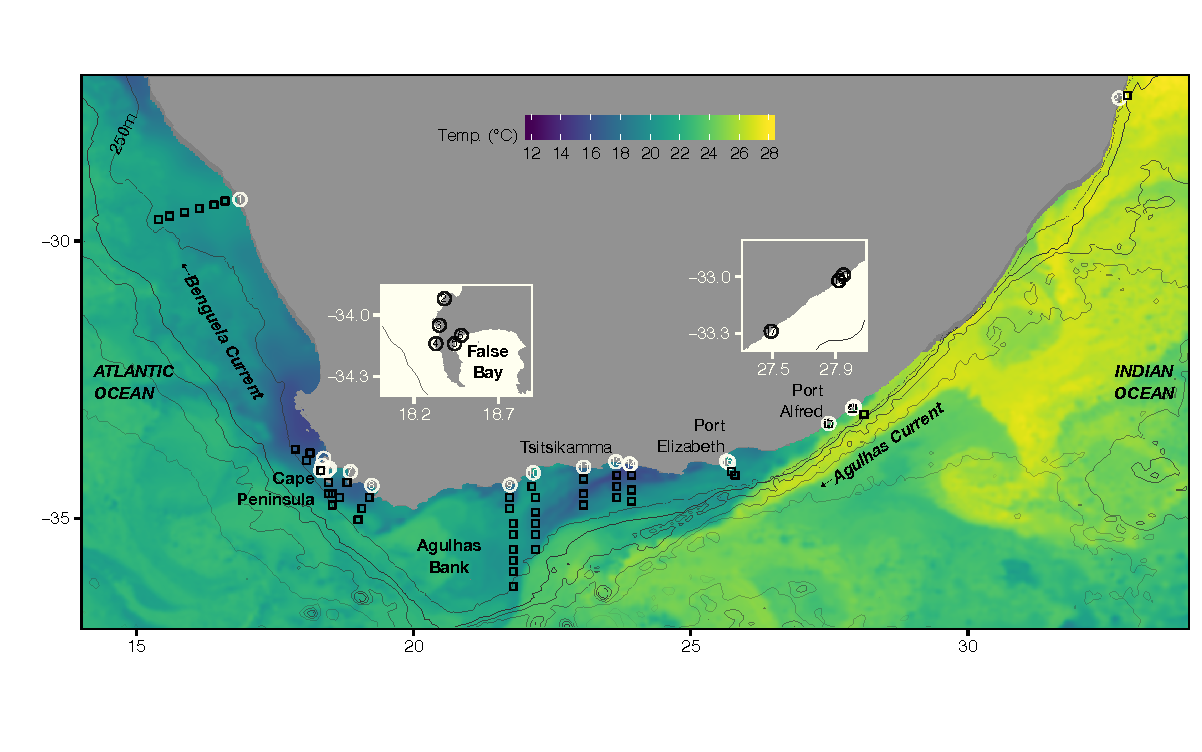
\includegraphics[width=1.0\textwidth]{figure1_1km_inset_map_labeled.pdf}
\caption{Map of southern Africa showing the bathymetry (only the 250m isobath is labelled), the location of the \emph{in situ} thermal time series shown with circles and approximations of the pixels used along the shore-normal transects from the daily \sfrac{1}{4}\degree~NOAA OISST \cite{Reynolds2007} shown with black boxes. The JPL G1SST 1 km blended SST field shows the state of the ocean on 2016-02-14; this image was selected as it clearly shows the full range of ocean processes around southern Africa. The Agulhas Current along the east coast of the country is visualized here in a yellowish colour as a jet of relatively warmer water projecting in a south-westerly direction, and hugging the continental shelf. The blueish patches north of the Cape Peninsula represent upwelled water. Some upwelled water may also be present around Sites 14 (Tsitsikamma) and 15--16 (Port Elizabeth). The inset maps show detail of the Cape Peninsula/False Bay area and the Hamburg region where site labels are obscured due to overplotting of symbols.}
\label{fig:Figure1}
\end{figure}

\subsection{Temperature data}
We use two sources of seawater temperature data. The first dataset is comprised of 127 records of \emph{in situ} temperature records of daily measurements for up to 40 years in duration with a mean duration of \emph{ca}. 19 years. Whereas these \emph{in situ} time series are generally shorter than the recommended 30 year minimum \citep{Hobday2016} and have some small amounts of missing data, it is our opinion that the benefit of using \emph{in situ} data over satellite data is that they give a better representation of the temperatures felt by coastal ecosystems as well as the thermal characteristics near the coast, a region where satellite SST measurements have been shown to perform poorly \citep[e.g.][]{Smale2009, Castillo2010}. In a South African context, \citet{Smit2013} have shown that satellite SST data display a warm bias as large as 6\degree C over \emph{in situ} temperatures in the nearshore environment. In an attempt to compromise between the proscribed requirements in \citet{Hobday2016} of a 30 year minimum and making use of this valuable dataset, all time series under 10 years in duration were eliminated. We found 10 years to be the minimum duration required in order to generate a robust estimate of the climatology required for the identification of MHWs and MCSs. Next, the remaining time series were further screened and those missing more than 10\% of their daily values were removed, leaving a total of 21 time series. Care was taken to select continuous series with as few as possible consecutive missing values, since having regions in the data with more than two consecutive missing data points interferes with the identification of the anomalous events (see below). These stations were classified into three coastal sections defined by properties of their oceanography and biogeography \cite{Smit2013}. Details on the selected time series, including location, duration, and the coastal sections they were aggregated into may be found in \Cref{tableS1} and the site localities are displayed spatially in \Cref{fig:Figure1}.

The second set of temperature data used in this study are the daily \sfrac{1}{4}\degree~NOAA optimally interpolated sea surface temperature \citep[OISST;][]{Reynolds2007} derived from the Advanced Very High Resolution Radiometer (AVHRR). To compare the offshore mesoscale (OISST dataset) extreme events against those along the coast (\emph{in situ} dataset), shore-normal transects were drawn from each of the 21 sites extending to the 200m isobath. Temperature values from the OISST data were then extracted at each of the roughly 25~\texttimes~25 km pixels along these transects, shown as black boxes in \Cref{fig:Figure1}. Where the shelf was less than 25 km wide (Sites 17--21) the nearest `ocean pixel' to the \emph{in situ} time series coordinate was used. It was decided to use mean temperatures along these shore-normal transects as they better represent the mesoscale temperatures we were interested in comparing against the coastal events, rather than simply using the nearest OISST pixel, as this would only draw a comparison between the two different data types at the coast, and not the mesoscale activity in the ocean. The individual time series within each pixel of each transects were then averaged to create 21 time series to match against those calculated for the \emph{in situ} sites. These 21 OISST time series could then be analysed for MHWs (MCSs) in the same way as the \emph{in situ} data (see below). Note that the OISST time series had valid data covering 1982--2015 which did not match exactly the coverage by individual \emph{in situ} sites.

\subsection{Defining and calculating MHWs and MCSs}
MHWs are defined here following \citet{Hobday2016} as ``discrete prolonged anomalously warm water events in a particular location.'' MCS are defined in the same manner as MHWs with the exception of being ``anomalously cold water events''.

First, a climatological mean and 90th and 10th percentiles were calculated for each day of the year by pooling all data within an 11-day window across all years. MHWs (MCSs) were detected as periods of time when temperatures exceeded the 90th (10th) percentile for at least five days. The implication was therefore that MHWs (MCSs) could develop outside of the warm (cold) season (i.e. winter (summer) months). Since our \emph{in situ} time series were of differing durations we calculated the climatology over all available years; in the case of the OISST data, climatologies were calculated over a fixed 33-year base period (1982--2015). Furthermore, discrete events with well-defined start and end dates but with `breaks' between events lasting $\leq$2 days followed by subsequent $\geq$5 day events were considered as continuous events. After the events were defined, a set of metrics (\Cref{table1}) were calculated including maximum and mean intensity (measured as anomalies relative to the climatological mean, in \degree C), duration (days from start to end dates, in days), and cumulative intensity (the integrated intensity over the duration of the event analogous to degree-heating-days, in \degree C). Although MCS intensities are calculated as negative values (i.e. anomalies) they are reported here as absolute values.

\begin{table}[]
\caption{\small Metrics of MHWs and their descriptions as used by \citet{Hobday2016}. In the case of MCSs, values are calculated with respect to the 10th percentile and absolute intensity values are reported.}
\label{table1}
\centering
\tiny
\begin{tabular}{ll}
\toprule
 Name [unit] & Definition \\
 \midrule
  Count [no. events per year] & \emph{n}: number of MHWs per year \\
  Duration [days] & \emph{D}: Consecutive period of time that temperature exceeds the threshold \\
  Maximum intensity [\degree C] & \emph{i\textsubscript{max}}: highest temperature anomaly value during the MHW \\
  Mean intensity [\degree C] & \emph{i\textsubscript{mean}}: mean temperature anomaly during the MHW \\
  Cumulative intensity [\degree C] & \emph{i\textsubscript{cum}}: sum of daily intensity anomalies over the duration of the event \\
  \bottomrule
  \end{tabular}
\end{table}

A Python script \citep[https://github.com/ecjoliver/marineHeatWaves; see][]{Hobday2016} was used to calculate the individual MHWs for both the \emph{in situ} and OISST time series. The script was modified to permit the calculation of MCSs. After the individual events were recorded, mean annual values for the metrics seen in \Cref{table1} were created for each year of each times series. This provided two different sets of measurements for the extreme events that will be referred to specifically throughout this paper. `Annual' data refer to the annual means of events for each year of each time series whereas `event' data refer to the individually calculated events within each time series.

Because MHWs (MCSs) are calculated by percentiles, rather than absolute definitions such as periods with temperatures above an arbitrary fixed temperature threshold, any time of year could be shown to be experiencing a MHW (MCS). This is an important consideration as unusually warm waters occurring during the winter months of a year, the time when many species need cold water for effective spawning/spore release, can have a negative effect on the recruitment success of that population for the year \citep{Wernberg2011}.

\subsection{Detecting co-occurrence of coastal and offshore events}
In order to better understand the potential impact mesoscale phenomena have on coastal events, the proportion of co-occurrence between the MHWs (MCSs) found within each time series between the two datasets was calculated. This was initially done by taking each event (warm and cold) within an \emph{in situ} time series and looking for an event occurring within the OISST time series at the same site within a certain period of time before the \emph{in situ} date. These co-occurrence proportions were used to describe how often the mesoscale oceanography off the coast led the extreme events occurring along the coast. All events occurring on dates outside of the dates occurring within the matching time series were removed from this calculation. The sum of events found to occur within the same time frame was then divided by the total number of \emph{in situ} events that occurred during the time period shared with the OISST data (which varies from station to station) to produce a co-occurrence proportion. The proportions of co-occurrence were then recalculated controlling for the size of the lag window used when comparing the two different datasets for concurrent events, as well as the directionality used for this comparison. In other words, a range of window sizes from 2-14 were used for each site to see how far apart events generally occurred and the lag period used was also applied only after the \emph{in situ} date, as well as both before and after the date, effectively doubling the range of the lag. This allowed us to see how often the \emph{in situ} event led the mesoscale event as well as seeing broadly the amounts of co-occurrence occurring between the two data sets.

Besides controlling for the duration and direction of lag, the size of the events themselves (ranked by cumulative intensity) was compared. This was accomplished by controlling the pool of events with which to compare the datasets per site in steps of 10th percentiles. This progressively removed smaller events until only the larger events were being compared. This allowed us to track the co-occurrence of only the largest events, reducing the overall proportion of co-occurrence found within each site as caused by the smaller events occurring at similar times as large events.

The top three MHWs (MCSs) for each \emph{in situ} and OISST time series as defined by cumulative intensity were also noted in order to visually compare the co-occurrence of events in detail, both within and between the different datasets.

Given that the anthropogenic forcing of climate change is predicted to increase the temperature of most of the ocean over time, it stands to reason that, as a function of the 90th and 10th percentiles, one would expect to see the larger MHWs near the end of the time series, and the larger MCSs near the beginning. This can be tracked visually by looking at the top three warm and cold events for each time series. Given that the OISST time series are greater than 30 years in duration it is possible to discern the long term trends within the data apart from the noise of any inter-decadal patterns (Schlegel and Smit, in review). Using a simple linear model, the decadal trend in the annual occurrence of MHWs and MCSs was calculated for all of the OISST data as well as the \emph{in situ} time series that were over 30 years long. The shorter time series simply had the proportion of MHWs or MCSs in the first half of the time series compared against those in the second half to show if there were more or fewer.

\section{Results}

\subsection{Event metrics}
Looking for differences in the metrics of MHWs and MCSs between datasets and between coasts (\Cref{table2}), a series of general linear hypotheses \citep{Hothorn2008} revealed significant differences in the frequency of MHWs and MCSs between the \emph{in situ} and OISST datasets, with the OISST dataset displaying more events of each kind (MHWs: \emph{t}=-5.37, \emph{p}<0.01; MCSs: \emph{t}=-5.28, \emph{p}<0.01). The number of hot events is neither more nor less than the number of cold events irrespective of dataset analysed. Considering the difference in MHWs or MCSs between coasts, differences were not found for the \emph{in situ} nor the OISST datasets.

MHWs and MCSs detected in the OISST dataset are of longer duration than in the \emph{in situ} dataset (MHWs: \emph{t}=-2.34, \emph{p}<0.05; MCSs: \emph{t}=-3.31, \emph{p}<0.01). Comparing coasts within the \emph{in situ} dataset, cold events are shorter along the east than along the south (\emph{t}=5.41, \emph{p}<0.01) or west coasts (\emph{t}=2.06, \emph{p}<0.05); the warm events show the same response, with the duration along the east coast being shorter than along the south (\emph{t}=3.79, \emph{p}<0.01) or west (\emph{t}=2.67, \emph{p}<0.01) coasts. MCSs are also of shorter duration along the east coast compared to the south coast in the OISST dataset (\emph{t}=2.83, \emph{p}<0.01), while MHWs follow the same pattern that emerged in the \emph{in situ} data (east \emph{vs.} south: \emph{t}=6.01, \emph{p}<0.01; east \emph{vs.} west: \emph{t}=3.79, \emph{p}<0.01). Contrasting the duration of MHWs with that of MCSs within coast and dataset, the duration of the two event types is identical, except for in the OISST dataset along the east coast where cold events last longer (\emph{t}=-2.70, \emph{p}<0.01).

The \emph{in situ} dataset yielded more intense MHWs (\emph{t}=19.80, \emph{p}<0.01) and MCSs (\emph{t}=14.19, \emph{p}<0.01) than the OISST dataset. Looking at the difference in intensity of events within dataset, MCSs are more intense than MHWs in the OISST dataset (\emph{t}=-4.10, \emph{p}<0.01). There are also differences in the intensity of MHWs and MCSs between coasts within a dataset. Considering the \emph{in situ} data, the intensity event types is greater along the south coast for both MHWs (south \emph{vs.} east: \emph{t}=-2.58, \emph{p}<0.01; south \emph{vs.} west: \emph{t}=3.28, \emph{p}<0.01) and MCSs (south \emph{vs.} east: \emph{t}=5.48, \emph{p}<0.01; south \emph{vs.} west: \emph{t}=-6.66, \emph{p}<0.01). More intense MCSs were detected in the OISST dataset on the south coast compared to the east (\emph{t}=-2.15, \emph{p}<0.05), while MHWs were less intense along the east compared to the south (\emph{t}=3.01, \emph{p}<0.01) or west (\emph{t}=2.18, \emph{p}<0.05) coasts. Focussing on differences between coasts but within a dataset, MHWs emerging from the \emph{in situ} dataset are more intense than their cold counterparts along the west (\emph{t}=4.48, \emph{p}<0.01) and east (\emph{t}=3.06, \emph{p}<0.01) coasts, but MCS are more intense compared to MHWs along the south coast (\emph{t}=-5.66, \emph{p}<0.01). A coastal difference in intensity of cold and warm events is only seen along the east coast (\emph{t}=-4.36, \emph{p}<0.01) in the OISST dataset.

The mean annual statistics shown in \Cref{table2} give a broad overview of the events occurring along the coast; however, examining the largest MHWs and MCSs better aids in our understanding of which coastal sections show the most intense events. The ranking of these events is based on the cumulative intensity metric as explained in \Cref{table1}. To calculate the mean cumulative intensity of all events it was necessary to use the individual event data, and not the annual mean data used for \Cref{table2}. Doing so for MHWs from both datasets we see that there is a significant difference (\emph{t}=7.68, \emph{p}<0.01) in the mean±sd cumulative intensities with the \emph{in situ} dataset (26.11±24.37\degree C) having greater cumulative intensities than the the OISST dataset (18.65±15.10\degree C). The absolute mean±sd MCS cumulative intensities between the two datasets are also significantly different (\emph{t}=2.99, \emph{p}<0.01) with the \emph{in situ} events (26.45±24.25\degree C) being greater than the the OISST events (23.17±23.49\degree C).

\begin{table}[]
\centering
\caption{\small The mean±sd values for event count, duration and mean intensity from the annual data for MHWs and MCSs for each coastal section as calculated from the \emph{in situ} (A)  and OISST (B) time series. The aforementioned annual data were averaged across all years for all time series within each respective coast to produce the mean±sd values shown. Lower case letters indicate if any of the coastal sections differ \emph{within} the same dataset \emph{and} event type, with metrics sharing the same letter being statistically indistinguishable from one-another (i.e. MHW or MCS). Upper case letters indicate if the coastal sections differ \emph{between} the datasets, but \emph{within} coast \emph{and} event type.}
\label{table2}
\begin{tiny}
\begin{tabular}{lccccccc}
\toprule
& \multicolumn{3}{c}{MHW} & \phantom{abc} & \multicolumn{3}{c}{MCS} \\
\cmidrule{2-4} \cmidrule{6-8}
coast & count [n] & duration [days] & mean intensity [\degree C] && count [n] & duration [days] & mean intensity [\degree C days] \\
\midrule
{\bf{A} --- \emph{in situ}} \\
all & 1.6±1.8\textsuperscript{-A} & 9.3±5.1\textsuperscript{-A} & 2.65±0.79\textsuperscript{-A} && 1.5±1.7\textsuperscript{-A} & 9.0±5.1\textsuperscript{-A} & 2.79±1.09\textsuperscript{-A} \\
west & 1.8±1.9\textsuperscript{aA} & 9.1±3.9\textsuperscript{aA} & 2.86±0.90\textsuperscript{aA} && 1.5±1.9\textsuperscript{aA} & 8.5±5.2\textsuperscript{aA} & 2.32±0.58\textsuperscript{aA} \\
south & 1.5±1.8\textsuperscript{aA} & 9.8±6.1\textsuperscript{aA} & 2.50±0.65\textsuperscript{bA} && 1.5±1.6\textsuperscript{aA} & 9.7±5.5\textsuperscript{aA} & 3.08±1.22\textsuperscript{bA} \\
east & 1.5±1.7\textsuperscript{aA} & 7.7±2.2\textsuperscript{bA} & 2.85±0.89\textsuperscript{aA} && 1.6±1.6\textsuperscript{aA} & 7.1±1.9\textsuperscript{bA} & 2.37±0.67\textsuperscript{aA} \\
{\bf{B --- OISST}} \\
all & 2.2±2.1\textsuperscript{-B} & 10.2±5.4\textsuperscript{-A} & 1.72±0.33\textsuperscript{-B} && 2.2±2.6\textsuperscript{-B} & 10.2±5.1\textsuperscript{-B} & 1.83±0.52\textsuperscript{-B} \\
west & 2.1±1.8\textsuperscript{aA} & 10.9±6.7\textsuperscript{aA} & 1.75±0.41\textsuperscript{aB} && 2.3±2.7\textsuperscript{aA} & 9.8±6.6\textsuperscript{adA} & 1.87±0.61\textsuperscript{adB} \\
south & 2.2±2.1\textsuperscript{aB} & 10.6±5.5\textsuperscript{aA} & 1.74±0.29\textsuperscript{aB} && 2.1±2.7\textsuperscript{aB} & 10.7±5.0\textsuperscript{aA} & 1.79±0.45\textsuperscript{aB} \\
east & 2.5±2.3\textsuperscript{aA} & 8.3±2.4\textsuperscript{bA} & 1.64±0.33\textsuperscript{bB} && 2.2±2.2\textsuperscript{aA} & 9.4±3.4\textsuperscript{dA} & 1.93±0.61\textsuperscript{dB} \\
\bottomrule
\end{tabular}
\end{tiny}
\end{table}

\subsection{Patterns in mean cumulative intensity}

\begin{table}[]
\centering
\caption{\small The three largest MHWs and MCS per coast from the \emph{in situ} (A, B) and OISST (C, D) data. The coast column shows in which coastal section the event occurred. The site column gives the name of the site, as seen in \Cref{tableS1}, which gives the index number necessary to find it's location along the coast in \Cref{fig:Figure1}. The start date column gives the day on which the event began and the duration [days] column shows how many days the event lasted for. The mean intensity and cumulative intensity columns are explained in \Cref{table1}.}
\label{table3}
\begin{tiny}
\begin{tabular}{llcccc}
\toprule
coast & site & start date & duration [days] & mean intensity [\degree C] & cumulative intensity [\degree C days] \\
\midrule
\multicolumn{6}{c}
{\bf{\emph{in situ}}} \\
\multicolumn{6}{l}
{\bf{A --- MHW}} \\
west & Sea Point & 1996-01-04 & 40 & 3.08 & 123.20 \\
west & Sea Point & 2005-05-21 & 39 & 2.56 & 99.66 \\
west & Sea Point & 1975-12-30 & 38 & 2.62 & 99.41 \\
south & Muizenberg & 1999-12-01 & 98 & 3.17 & 310.30 \\
south & Mossel Bay & 1993-06-25 & 97 & 1.77 & 171.30 \\
south & Muizenberg & 1999-10-20 & 35 & 4.47 & 156.40 \\
east & Nahoon Beach & 1995-10-14 & 18 & 5.18 & 93.31 \\
east & Eastern Beach & 1985-12-27 & 19 & 3.33 & 63.18 \\
east & Orient Beach & 1990-06-25 & 12 & 3.80 & 45.59 \\
\multicolumn{6}{l}
{\bf{B --- MCS}} \\
west & Sea Point & 1990-06-23 & 44 & 2.88 & 126.60 \\
west & Sea Point & 1983-06-10 & 39 & 2.84 & 110.90 \\
west & Sea Point & 2000-11-28 & 23 & 3.70 & 85.04 \\
south & Muizenberg & 1984-07-14 & 63 & 2.92 & 183.70 \\
south & Muizenberg & 1992-03-24 & 56 & 2.78 & 155.60 \\
south & Ystervarkpunt & 2000-05-11 & 51 & 2.94 & 150.10 \\
east & Sodwana & 2004-02-12 & 17 & 3.25 & 55.20 \\
east & Orient Beach & 1984-03-31 & 13 & 3.73 & 48.44 \\
east & Orient Beach & 1995-12-6 & 15 & 3.01 & 45.13 \\
\multicolumn{6}{c}
{\bf{OISST}} \\
\multicolumn{6}{l}
{\bf{C --- MHW}} \\
west & Sea Point & 1992-01-21 &  39 & 2.96 & 115.60 \\
west & Hout Bay & 1992-01-20 &  36 & 3.15 & 113.50 \\
west & Kommetjie & 2004-10-29 &  53 & 2.03 & 107.40 \\
south & Knysna & 1992-05-3 &  50 & 2.41 & 120.40 \\
south & Fish Hoek & 2004-10-30 &  53 & 1.92 & 101.60 \\
south & Pollock Beach & 1994-03-27 &  31 & 3.19 & 99.05 \\
east & Nahoon Beach & 2006-10-21 &  25 & 1.81 & 45.34 \\
east & Eastern Beach & 2000-06-24 &  26 & 1.58 & 41.12 \\
east & Orient Beach & 2000-06-24 &  26 & 1.58 & 41.12 \\
\multicolumn{6}{l}
{\bf{D --- MCS}} \\
west & Kommetjie & 2010-12-13 &  54 & 3.92 & 211.90 \\
west & Hout Bay & 2010-12-25 &  41 & 4.06 & 166.30 \\
west & Sea Point & 2010-12-25 &  41 & 3.78 & 154.90 \\
south & Hamburg & 1984-02-5 &  65 & 3.91 & 254.20 \\
south & Storms River Mouth & 1982-03-13 &  60 & 2.79 & 167.30 \\
south & Tsitsikamma East & 1982-03-13 &  60 & 2.79 & 167.30 \\
east & Eastern Beach & 2010-12-26 &  32 & 2.90 & 92.85 \\
east & Orient Beach & 2010-12-26 &  32 & 2.90 & 92.85 \\
east & Eastern Beach & 1984-02-24 &  22 & 3.97 & 87.26 \\
\bottomrule
\end{tabular}
\end{tiny}
\end{table}

The three largest MHWs that occur within the \emph{in situ} dataset are all on the south coast (\Cref{table3}). The size of the south coast events are larger than those along the west coast, with the largest three MHWs from the east coast being the smallest. This is due in part to the events on the south coast having a greater duration than the other two coastal sections, which influences the cumulative intensity metric. As with the MHWs, the largest three MCSs from the \emph{in situ} data are also on the south coast (\Cref{table3}). The west coast has the next largest three events and the east coast the smallest. The south coast MCSs have a greater duration than the MCSs from the other coastal sections, but are less pronounced than that of the MHWs.

The pattern seen in the \emph{in situ} data of the largest MHWs and MCSs occurring on the south, west and east coasts respectively is not repeated with the OISST dataset. Whereas the single largest MHW occurs on the south coast in the OISST data, the three largest MHWs from the west coast are larger than the second and third largest events from the south coast (\Cref{table3}). The three largest MHWs from the east coast are again smaller than those from the other coasts. The largest MCSs for the south and west coasts from the OISST data are similarly show no clear pattern with no one coastal section having the three largest events as in the \emph{in situ} dataset. The east coast MCSs from the OISST dataset are however consistent in that they are again the smallest three events. All of the coastal sections in the OISST dataset show that at least two of their largest MCSs occurred at the same time at different sites. This is a level of co-occurrence that the \emph{in situ} data do not show.

A three-way ANOVA on the individual event data for both the \emph{in situ} and OISST data combined (i.e. as with the annual data) with three factors (coast, event type, dataset) yielded significant marginal effects and interactions between all factors (\emph{p}$\leq$0.03).

As well as having significantly different cumulative intensities, one can see in \Cref{fig:Figure2} that the three largest events occurring for each time series within the OISST dataset are often different from those seen in the \emph{in situ} dataset, but show a greater amount of co-occurrence with events detected at neighbouring coastal stations than the corresponding \emph{in situ} time series do.

\begin{sidewaysfigure}
\centering
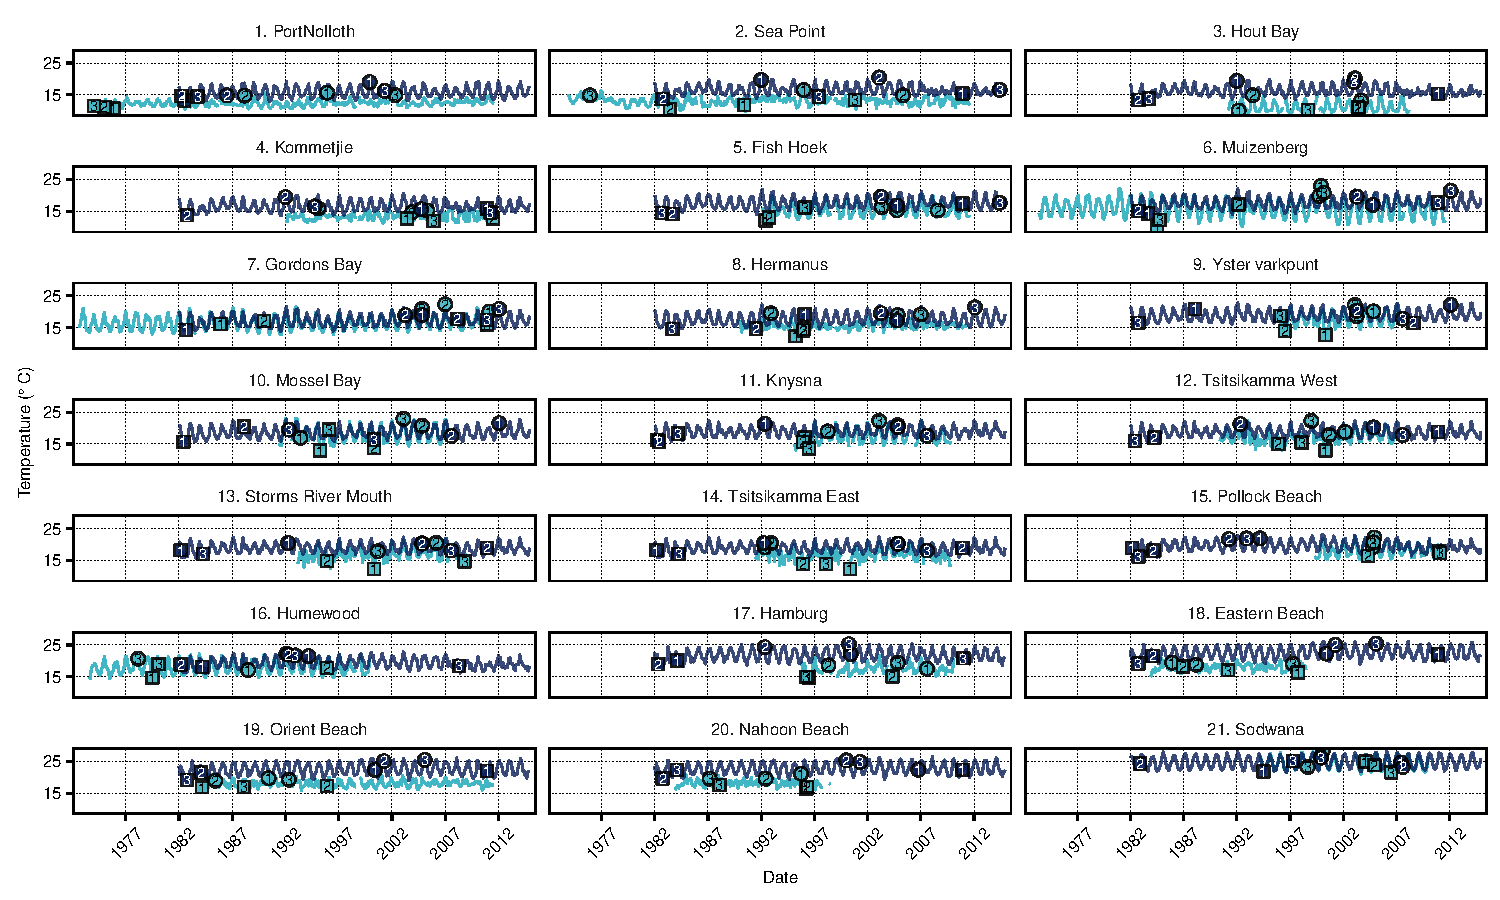
\includegraphics[width=1.0\textwidth]{figure2.pdf}
\caption{The daily temperature values for each \emph{in situ} time series (light blue) used in this study and the corresponding OISST time series (dark blue) extracted for comparison as seen in \Cref{fig:Figure1}. The top three MHWs are indicated by circles (with the rank inside) for each site as judged by greatest cumulative intensity. The top three MCSs for each site are indicated by squares (with the rank inside). Sites 1--4 represent the west coast (WC), sites 5--17 represent the south coast (SC) and sites 18--21 represent the east coast (EC). The coefficient of determination (R$^2$) values for the daily temperatures between each paired set of time series are displayed in the upper left corner of each panel.}
\label{fig:Figure2}
\end{sidewaysfigure}

The temperatures on the dates of the largest MHW and MCS for the west and south coasts from the \emph{in situ} data may be seen concurrently with the temperatures from the matching OISST time series in \Cref{fig:Figure3}. One may see that when the largest events were occurring in the \emph{in situ} data, the temperatures in the OISST data did not show similarly intense events.

\begin{figure}
\centering
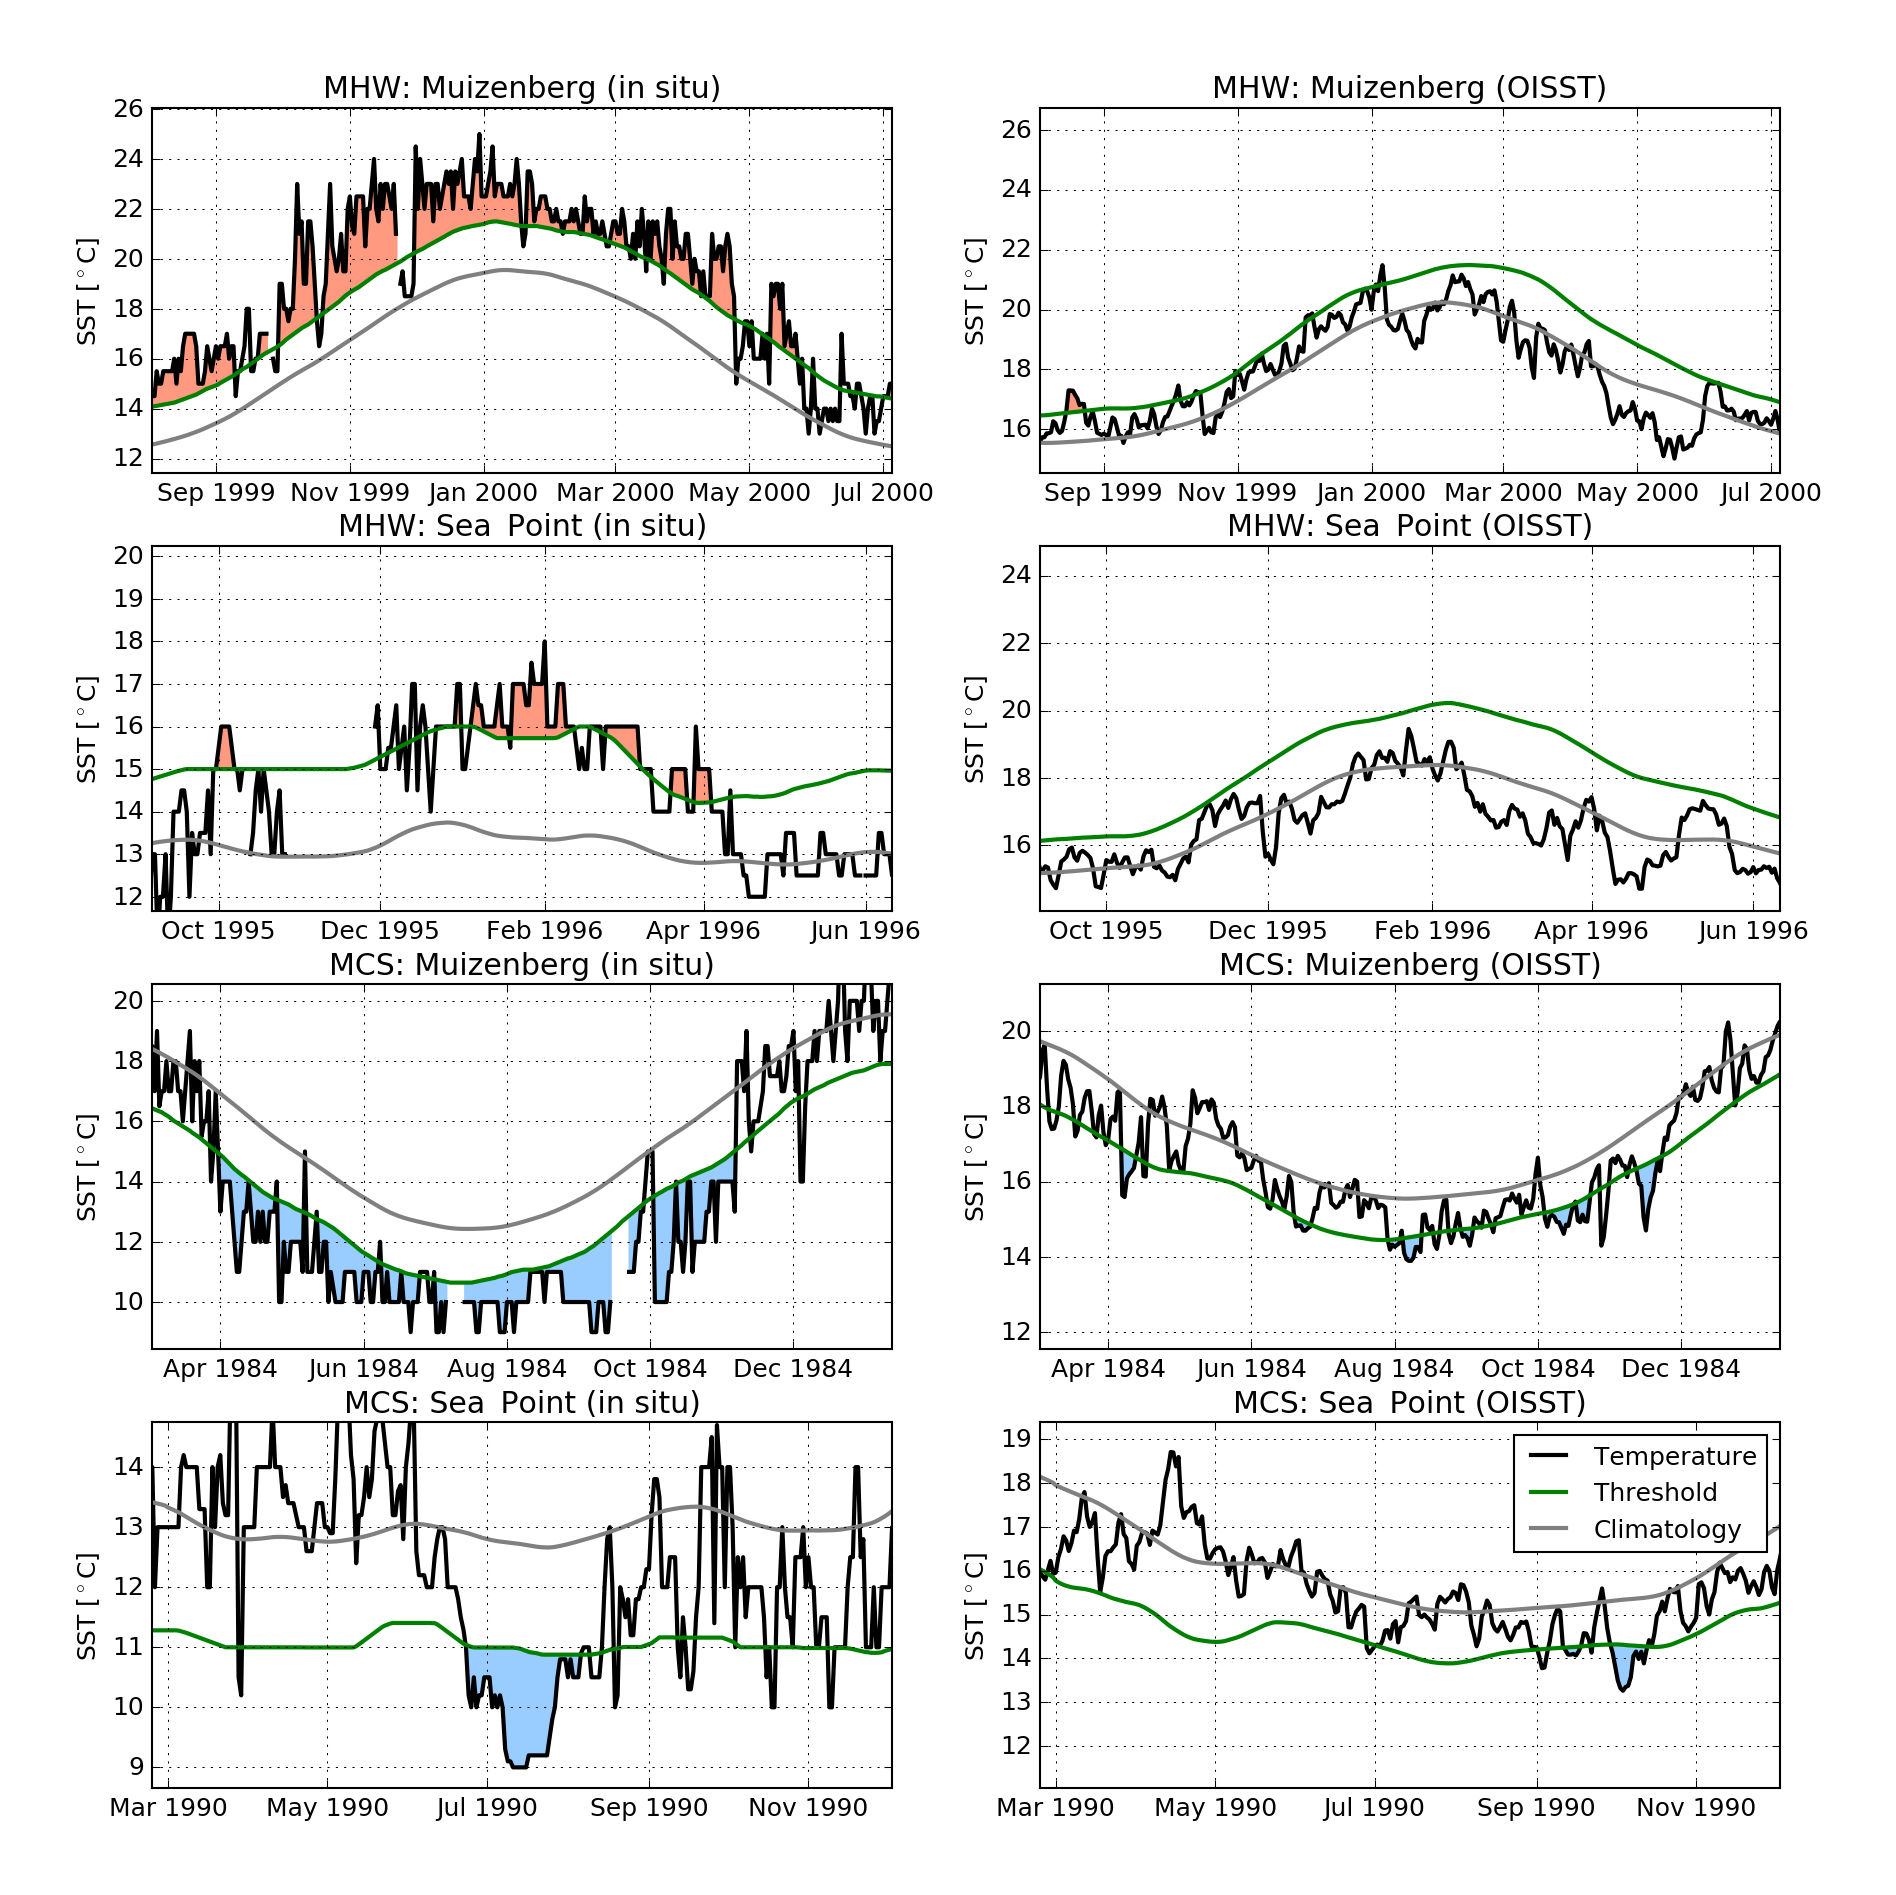
\includegraphics[width=1.0\textwidth]{figure3.png}
\caption{The temperature values from the \emph{in situ} and OISST data during the largest MHW and MCS from the south and west coasts respectively from the \emph{in situ} data. The left column shows the \emph{in situ} temperature values during the event while the right column shows the OISST temperature values occurring on the same dates. The top row shows the largest MHW that occurred on the south coast while the second row shows the largest MHW that occurred on the west coast. The bottom two rows show the largest \emph{in situ} MCS that occurred on the south and west coasts respectively.}
\label{fig:Figure3}
\end{figure}

\subsection{Co-occurrence rates}
The proportion of co-occurrence found for MHWs and MCSs between the datasets for each site may be seen in \Cref{fig:Figure4} and \Cref{fig:Figure5} respectively. When using the lag windows before and after the \emph{in situ} event and comparing all events we see that as the width of the lag window increases from 2 to 14 days the mean proportion of co-occurrence for all sites increases linearly for MHWs (0.09 to 0.38) and MCSs (0.10 to 0.30). Using these same constraints we see that south coast sites have the largest mean increase in co-occurrence for MHWs (0.10 to 0.45) and MCSs (0.11 to 0.34), whereas the west coast sites show the smallest increase for MHWs (0.07 to 0.28) and MCSs (0.08 to 0.19). With all variables controlled for in the same manner, the co-occurrence rates between the different coastal sections are not significantly different for MHWs or MCSs at 2 day nor 14 day lags (\emph{p}$\geq$0.12).

The directionality of the lag window also affects the co-occurrence of events. Comparing all events within a 14 day lag window before the \emph{in situ} event gives higher mean±sd rates of co-occurrence for MHWs (0.22±0.13) than for the same lag window after the \emph{in situ} event for MHWs (0.18±0.10). This same comparison for MCSs shows that the lag window before the \emph{in situ} event (0.16±0.09) has slightly lower rates of co-occurrence than the lag window after the \emph{in situ} event (0.17±0.08). When the smaller events were screened from comparison and only the largest half of the events used (50\textsuperscript{th} percentile), the difference in mean±sd co-occurrence proportions for MHWs event lessens at 0.16±011 before the \emph{in situ} event and 0.15±0.12 after. The mean±sd co-occurrence proportion of MCSs at this level is less when using a lag window before the \emph{in situ} event at 0.05±0.08 than for a lag window after at 0.08±0.08.

There is no co-occurrence for the largest MCSs between the datasets, whereas four of the 21 time series show co-occurrence for their most extreme MHWs (\Cref{fig:Figure4}). Interestingly, all four time series are on the south coast and three of the four show co-occurrence for their largest MHW when the \emph{in situ} event preceded the OISST event.

\begin{figure}
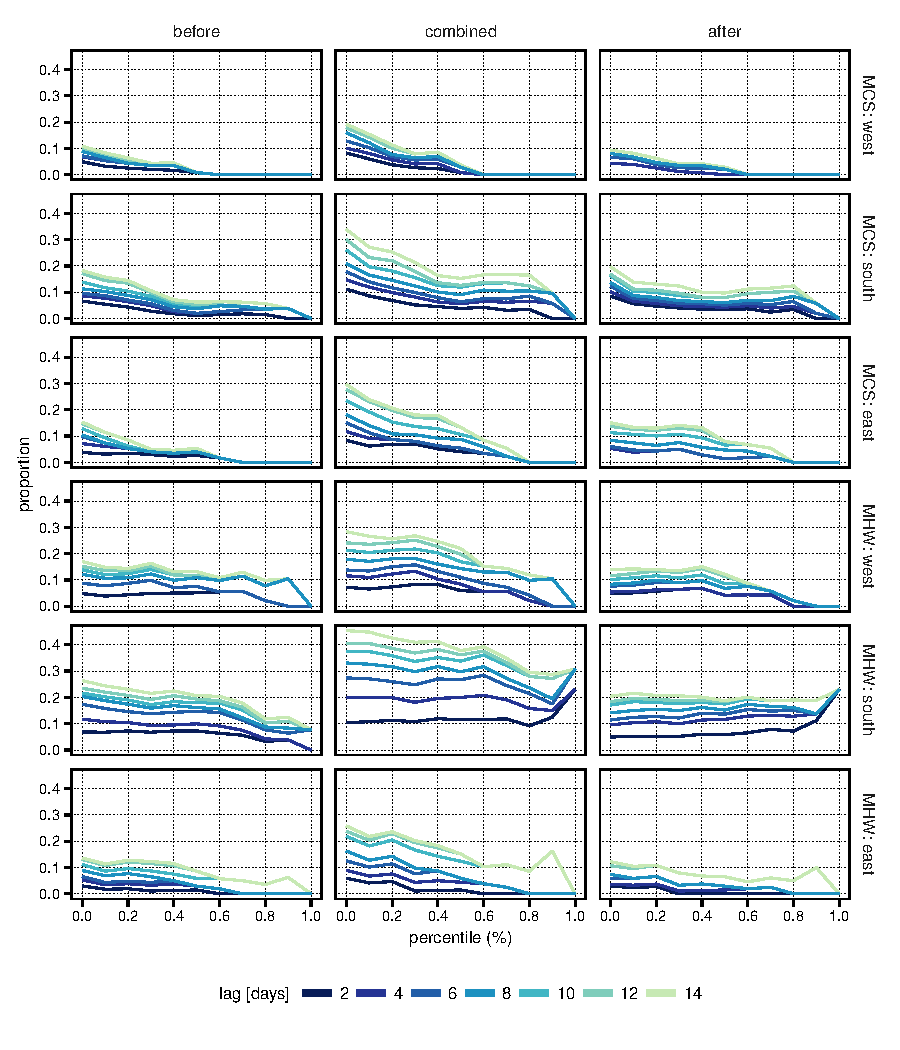
\includegraphics[width=1.0\textwidth]{figure4.pdf}
\caption{Proportion of MHW co-occurrence between \emph{in situ} and OISST datasets for each site where sites 1-4 represent the west coast (WC), sites 5-17 the south coast (SC) and 18-21 the east coast(EC). Columns denoted with ``before'' show the proportion of co-occurrence when events in the OISST data occurred on or before the dates of the \emph{in situ} events. The columns denoted with ``after'' show the proportion of co-occurrence when OISST events occurred after the \emph{in situ} event dates. The $x$-axis indicates the size of the events, based on percentiles, used for calculating the co-occurrence proportions. The days of lag used, from 2-14, are shown here in diminishing shades of red. The numbers above each panel show th ID number for each site. The names of the sites that relate to these ID numbers may be found in \Cref{fig:Figure2} and \Cref{tableS1}.}
\label{fig:Figure4}
\end{figure}

\begin{figure}
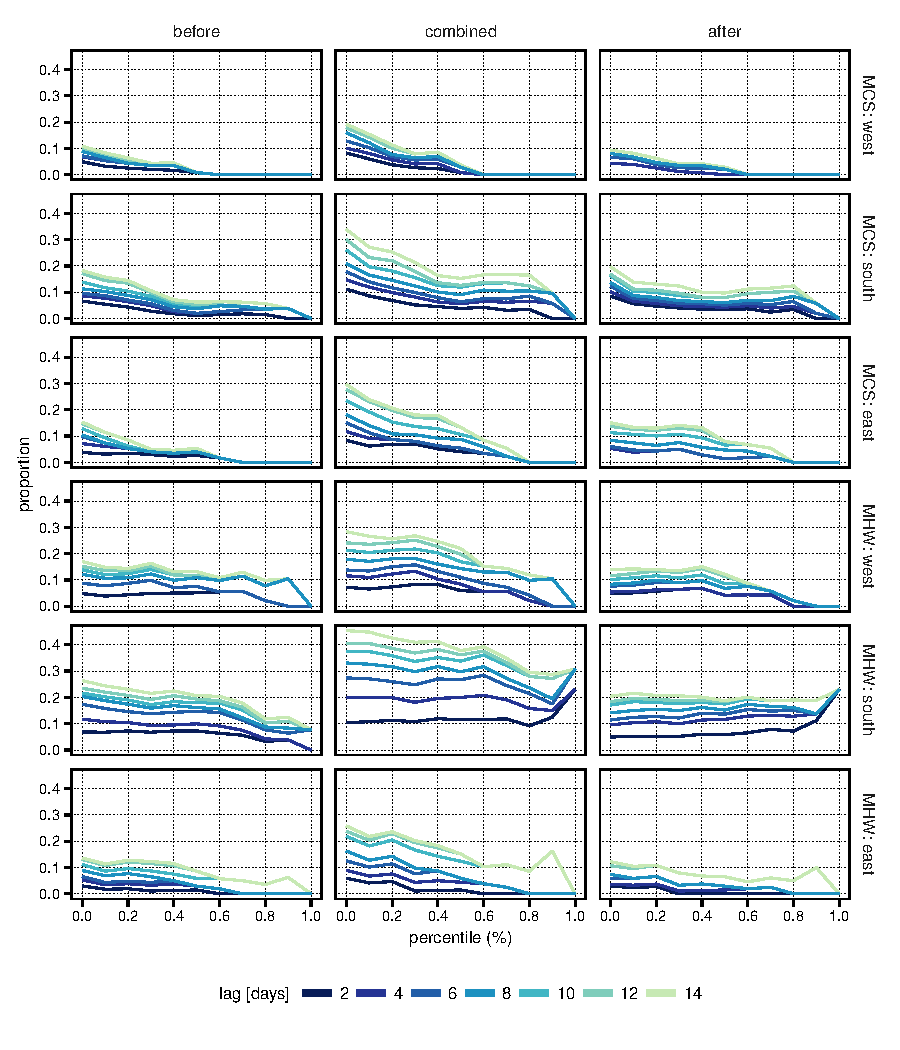
\includegraphics[width=1.0\textwidth]{figure5.pdf}
\caption{Proportion of MCS co-occurrence between \emph{in situ} and OISST datasets for each site as seen for MHWs in \Cref{fig:Figure4}. The days of lag are shown here in diminishing shades of blue.}
\label{fig:Figure5}
\end{figure}

\subsection{Decadal trends in MHWs and MCSs}
In order to calculate the decadal trends in MHW and MCS count, linear models were fitted to the annual count values for each >30 year time series. The slope of this line indicate whether after >30 years MHWs/MCSs are increasing or decreasing. As the OISST data set is over 30 years in duration, decadal trends were calculated for each OISST time series. We see that the mean±sd decadal trend for MHW occurrence in the OISST dataset is 0.5±0.3~dec$^{-1}$ across all sites and -0.7±0.6±~dec$^{-1}$ for MCSs. The decadal trends in MHW occurrence increase as one moves from the colder Benguela fed west coast to warmer Agulhas driven east coast with the mean±sd decadal MHW trend on the west coast being 0.3±0.3~dec$^{-1}$, the south coast being 0.5±0.3~dec$^{-1}$ and the east coast at 0.6±0.2~dec$^{-1}$. Just as MHWs are occurring more frequently per decade on the east coast than the west, the frequency of MCSs is decreasing more on the east coast than the west. The decadal trend in MCSs on the west coast is -0.1±0.6~dec$^{-1}$, -0.8±0.5~dec$^{-1}$ on the south coast and -0.9±0.2~dec$^{-1}$ on the east coast. \todo{How about tabulating these, and including also the \emph{p}-values, \emph{R}\textsuperscript{2}, etc.? I am working on this.-Rob}

Of the 21 \emph{in situ} time series, only four of them reach the >30 year requirement. Of these four time series the mean±sd decadal trend for MHWs is 0.3±0.5~dec$^{-1}$ and -0.1±0.5~dec$^{-1}$ for MCSs. There are two sites from the west coast and two from the south, excluding the east coast from a possible calculation of decadal change for \emph{in situ} MHWs and MCSs. The mean±sd decadal trend for MHWs (MCSs) on the west coast is 0.1±0.5~dec$^{-1}$ (-0.2±0.7~dec$^{-1}$) and 0.5±0.5~dec$^{-1}$ (0.1±0.4~dec$^{-1}$) on the south.

For the remaining 17 \emph{in situ} time series we calculated the sum of the annual count of both warm and cold events in the first and second halves. Comparing these results produced a proportion value that could then be used as an indicator as to how much more often MHWs or MCSs occurred in the second half of the time series \emph{vs,} the first. \todo{How about an ANOVA as a formal test for differences? I have calculated this and am now considering how to reword this paragraph.-Rob} The mean±sd proportion of MHWs occurring in the second half of the shorter time series was 1.7±1.3, whereas the proportion of MCSs was 0.8±0.6, suggesting that more of the MHWs occur in the second half of time series, and \emph{vice versa} for the MCSs. The shorter time series on the south coast show the pattern of having more MHWs in the second half of the time series at 2.1±1.4 and fewer MCSs in the second half at 0.5±0.3. The short west coast time series also has more MHWs in the second half at 1.5±0.6, but it also has more MCSs at 1.8±0.6. The east coast has fewer MHWs at 0.7±0.4 in the second half of the shorter time series with the proportion of MCSs being roughly split between the first and second half of the time series at 1.0±0.8.

\subsection{Offshore MHWs and MCSs}
When one languidly casts their gaze away from the coast and out towards the boundless expanse of ocean around southern Africa the mesoscale patterns as they occur independent of the continent may be more readily seen. \Cref{fig:Figure6} shows the mean count, duration and intensity of each pixel from the OISST dataset as derived from the annual data. The most MHWs occur well south of the tip of the continent whereas some of the most frequent MCS activity may be found directly against the west coast. This helps to explain the finding that MHWs were shown to be longer and more intense in the \emph{in situ} dataset, whereas the OISST dataset shows MCSs to be longer and more intense. As for the duration of events, it is clear from \Cref{fig:Figure6} that the MHWs and MCSs detected in the Agulhas current are relatively short-lived. Almost all of the pixels that show events in the upper range of the durations detected occur well away from the coast, too. This explains why the events in the \emph{in situ} data have a greater duration. As for the intensity of offshore events, the west and south coasts are shown to have centres of intensity very near the shore whereas the east coast generally does not. The most intense events detected in the OISST data are found along or south of the south coast, corroborating the finding that the south coast has the greatest proportion of co-occurrence amongst the three coastal sections.

\begin{figure}
\centering 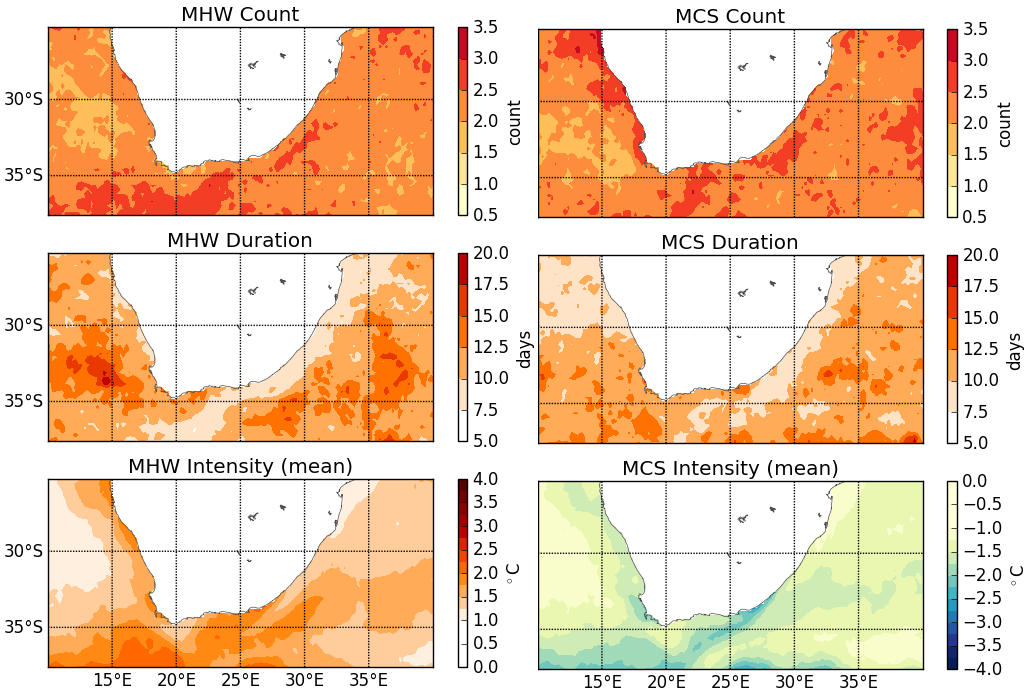
\includegraphics[width=1.0\textwidth]{MHW_MCS_mean.png}
\caption{Mean values from the annual data of each pixel from the OISST dataset around southern Africa. The first second and third rows show the mean count, duration (days) and intensity (\degree C) respectively of MHWs in the first column and MCSs in the second. The annual event values within each pixel were meaned to create one final value with which each pixel is populated. The `MCS Intensity (mean)' panel shows the intensity of the MCSs in negative values, not absolute values.}
\label{fig:Figure6}
\end{figure}

Whereas the mean count, duration and intensity of MHWs and MCSs offshore are telling, the picture is not complete without also considering the trend in these metrics, too. One may see in \Cref{fig:Figure7} that the count, duration and intensity of MHWs have almost exclusively been increasing throughout the studied regions of the Indian and Atlantic oceans. The count of MCS has been decreasing most rapidly along the coast of southern Africa with a couple of notable exceptions near Port Elizabeth and north of the Cape Peninsula where the count of MCSs have been increasing very near to the coast. The duration of MCSs is seen to generally increase further offshore with most of the nearshore changing little or decreasing. The intensity of MCSs is either changing little near the coast or is increasing dramatically, as seen in the dark blue spot north of the Cape Peninsula in the ``MCS Intensity (mean) Trend'' panel in \Cref{fig:Figure7}. This means that a consistent >30 year trend in extreme cold events, more so than anywhere else in this region of the ocean, has been acting on the coastal waters here.

\begin{figure}
\centering 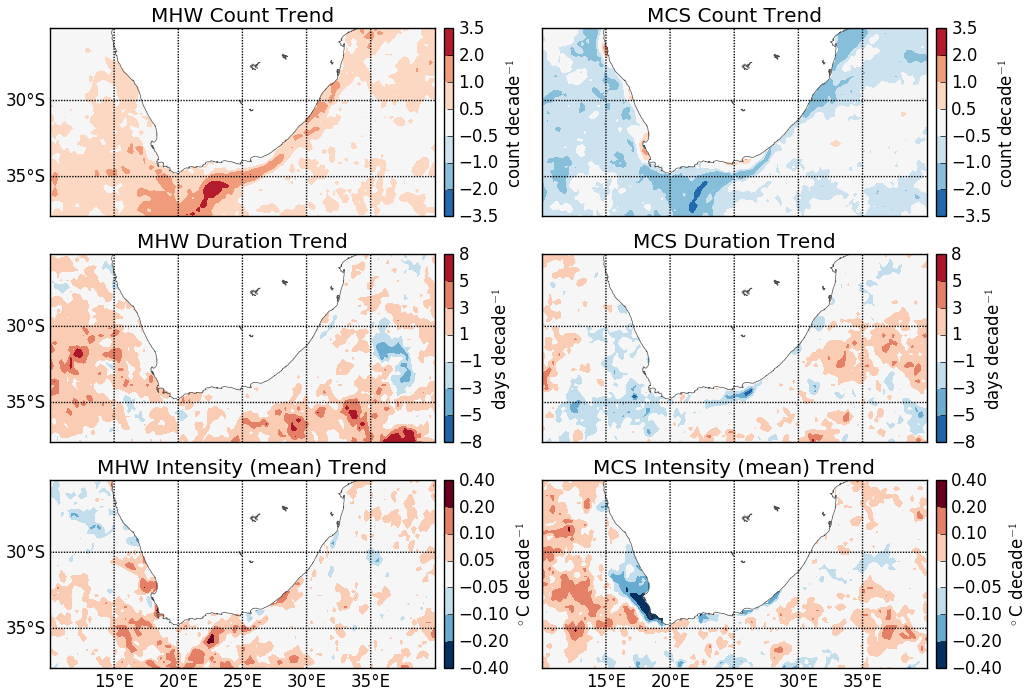
\includegraphics[width=1.0\textwidth]{MHW_MCS_trend.png}
\caption{Decadal trend values calculated from the annual OISST data around southern Africa. The decadal trends were calculated by fitting a linear model to the annual data of each pixel for the relevant metrics and multiplying the slope of the line by 10. The panels are in the same position as \Cref{fig:Figure6}. The ``MCS Intensity (mean) Trend'' panel shows the trend in MCS intensity as negative values, not absolute values (e.g. dark blue regions mean the MCSs are getting stronger, not weaker).}
\label{fig:Figure7}
\end{figure}

\section{Discussion}
Our results clearly show that MHWs and MCSs detected in two fundamentally different kinds of datasets display markedly differing metrics regarding the events' timing, frequency, duration and intensity. These differences appear to be related to the nature and variability of physical oceanographic processes at broad- and local-scales, and the coupling of the processes across these scales. These finding illustrate how a study of the properties of anomalous events can provide novel insights into drivers of the thermal regime along coastlines, and can be used to arrive at a mechanistic understanding of the nature and origin of MHWs (MCSs), which under a regime of climate change will become the major mode of perturbation to marine ecosystems and the marine living resources and coupled ecosystem services we derive from these systems. This analysis would not have been possible had it not been for the recent framework of \citet{Hobday2016}, which has enabled the calculation of objective, quantitative metrics for the comparison of anomalous thermal events across scales, location and time. However, \citet{Hobday2016} noted that their definition does not make assumptions about the drivers of heatwaves, nor does it hint at any ecological effects. We also draw no conclusions about the consequences of the events detected in our study, but we show how a careful analysis of events in contrasting datasets may yield information about the underlying drivers of those events. \todo{Are we achieving this?}

\subsection{Relation between local- and broadscale MHWs and MCSs}
The difference between the \emph{in situ} and OISST datasets is striking. We anticipated a large degree of coupling between the anomalously warm events manifesting in datasets that encapsulate local- and broad-scale patterns, as represented by the \emph{in situ} and OISST datasets, respectively. We found instead that the broad-scale dataset yields heatwaves that are more frequent and longer in duration, but less intense than its local-scale counterpart. Cold-spells, for which we expected a greater deal of decoupling between local- and broad-scale manifestations, indeed show evidence of such lack of coupling. MCSs are more frequently seen and last longer in the OISST data; however, the mean intensity of MCSs at the broad-scale is lower than at the coast. Furthermore, there is no difference in the frequency of MHWs and MCSs emerging at the two scales, but the duration and intensity of MHWs relative to MCSs across scale are modified by the section of the coast in which they occur. Taken at face value, these finding might suggest that both MHWs and MCSs are completely decoupled between coastal and offshore regions. A more in-depth assessment of the rates of coupling is provided later (see \emph{Co-occurrence rates}, below), and it shows that \emph{some} coupling is indeed present, particularly in MHWs.

An important outcome emerging from the above analysis is that the OISST dataset shows many weak events occurring often whereas the \emph{in situ} dataset shows fewer but more intense events. The interaction between frequency and duration is an important consideration, because this influences the cumulative intensity metric. This indeed emerges in mean cumulative intensities calculated for the MHWs and MCSs, which are highest in the \emph{in situ} data. Events near the coast are more intense overall. Heatwaves are ubiquitous throughout the world's oceans, but if this pattern of intensification of anomalous events at the coast holds true for different world regions, it creates interesting challenges for the management of marine living resources and ecosystems at the coast. The impact humans have on coastal ecosystems only excacerbates this looming threat. Over half of the world's countries have 80-100\% of their populations living within 100km of the coastline, where 21 of the largest 33 cities are also found and the population density of these coastal human aggregations is increasing much faster than anywhere else on the planet \citep{Martinez2007}. This increasing burden may be accelerating the decadal rate of warming seen in coastal waters \citep{Amos2013}, which would then likely further increase the already greater cumulartive intensity of the coastal MHWs over those seen further offshore.

Of the metrics presented in this paper, cumulative intensity (\degree C days) is the most important ecologically. As a product of the intensity and duration of an event, cumulative intensity may be used as an index to measure the threat of extreme events to coastal ecosystems. Research conducted on the damaging effects of extreme events \citep[e.g.][]{Wernberg2013} record the cumulative heat (\degree C days) above the seasonal average experienced by the coastal ecosystem in question. As the body of research on extreme events increases, these cumulative intensity values may be used to establish a global index of the thresholds for different ecosystems at which ecological perturbations, impairment or destruction has occurred. Combined with near real time monitoring, this metric may then be used to improve the decision making process on how when and how best to respond to unusually warm or cold bodies of weater.

We see that a large number of the events occurring between these two datasets are unrelated and that some other influence(s) may be having a more pronounced effect on the temperatures experienced at the coast than the ocean temperatures offshore. This conclusion is important in the light of the findings of \citet{Smit2013}, who found that there is a very strong mismatch in the temperatures recorded by thermal loggers installed \emph{in situ} at the coast (i.e. local-scale) compared to the measurement of the ocean's temperature from space (i.e. broad-scale). That study showed biases of up to +6 \degree C between the same local-scale dataset used here and AVHRR and MODIS Terra SST, with a strong spatial pattern. The insight emerging from the present study is that there are not only spatial influences affecting the mismatch between local- and broad-scale thermal patterns, but that there is a temporal component to these biases too. In other words, it is not possible to apply a constant and simple bias adjustment to the \emph{in situ} and SST time series used by \citet{Smit2013}. Such a deterioration of the offshore thermal signal in coastal waters is known to occur due to the local modifications of nearshore circulation patterns by headlands, embayments, influences of the bathymetry and other such perturbations that introduce eddies and fronts and a shoaling of the thermocline \citep{Okubo1973, Pingree1979, Wolanski1988, Black1990, Grundlingh1991, Graham1997}. These processes are by no means yet fully understood, and our understanding of physical oceanographic process remain weighted toward the mesoscale, as was noted by \citet{Graham1997} in the light of their study on upwelling shadows, another process responsible for the local modification of a phenomenon that is generally studied at the broad-scale. These local-scale deviations are know to affect coastal ecological processes, such as the transport, dispersal and settlement of larvae \citep{Pineda1994, McCulloch2003, Narvaez2004} and the dynamics of phytoplankton and nutrient delivery \citep{Graham1997, Pineda1994}, and it is likely that thermal patterns over similar scales will also have local significance for the biology of the nearshore region.

\subsection{MHWs and MCSs in different coastal sections}
Meaningful patterns of event metrics also emerge between coasts. The number of anomalously warm or cold events between coasts is not influenced by whether we are looking at coastal or offshore regions. Each coastal section is thus equally prone to experience a MHW or a MCS. Differences emerge in a comparison of the duration and intensity metrics, however. The east coast differs from the other two coastal sections in that MHWs and MCSs at both the local- and broad-scale are of shortest duration here; however, comparing the event duration between events, we see that in this regions the cold spells last longer than heatwaves. Furthermore, the east coast also displays the least intense MHWs but most intense MCSs of any coastal region along offshore portions of South Africa's coastline. This stretch of coastline is heavily influenced by the warm Agulhas Current, separated from the coast only by a very narrow and steep continental shelf, which abruptly expands into the >200km wide Agulhas Bank south of Port Alfred (\Cref{fig:Figure1}). The geography of the continental slope here interacts with the Agulhas current, independent of local atmospheric conditions, in two meaningful ways: i) the narrow margin of the continental slope alows upwelling on the shoreward side of this current to occur along the length of the east coast and ii) as the continental shelf expands, the speed and strength of the Agulhas current caries cold water up from the depths onto the shelf \citep{Lutjeharms2000}. If these events due indeed occur independent of atmospheric or meso-scale surface conditions, but are instead driven by the interaction between the Agulhas current and the continental shelf, it may explain why the duration of MCSs are significantly shorter on the east coast. This constant forcing however would also cause the events to break down more quickly to return to a normal stable state. This explains why the largest events, both hot and cold, recorded on the east coast are so much smaller than the other two coastal sections. The hydrodynamic properties of the Agulhas current prevent any prolonged temperature events from persisting.

The south coast differs fundamentally from the other two coastal sections in that it is dominated not by a strong current, such as the Agulhas or Benguela, but rather consists of a broad continental shelf on which the interplay of these two large bodies of water form the ephemeral border between two oceans. That the MHWs occurring within this coastal section should have significantly lower mean intensities than the other two coasts was unexpected as many of the \emph{in situ} time series here are recorded in shallow (~30m deep) embayments, allowing for thermal heating to have a marked effect, and further offshore sheer-edge forcing creates warm water eddies from the departure of the Agulas current from the Agulhas Bank that are then projected across the shelf \citep{Roberts2005}. The answer to these significantly smaller MHWs appears to lie in the increased variability of the south coast waters over the other two coastal sections. Due to the many different competing meso-scale phenomena here, the 90th percentile, over which an event must reach to be classsified as extreme, is proportionately higher than the other two coasts. Therefore the finding that the MHWs are significantly less intense is misleading. This conclusion is supported by the much lower standard deviation of MHWs on the south coast compared to the other two, showing that there was less possible range in temperatures that could be considered above the 90th percentile as the screening process was more demanding. The significantly more intense MCSs on the south coast are attributed to the much greater mean intensity of events around Tsitsikamma (Sites 12--14). Without these three sites the MCSs on the south coast are not significantly greater than the other two coasts. \citep{Roberts2005} hypothesised that a wind forced upwelling cell occurs near Tsitsikamma and the mean intensity of the events recorded here seems to support this.

The west coast does not show exceptional patterns in MHW and MCS metrics. At first glance, we were surprised to find that the mean intensity of south coast coastal MCSs are larger than those of the EBUS on the west coast. Upwelling systems are defined by periodic occurrences of cold water of deep origin near the coast and it seems intuitive to associate these with the cold-spells \hl{AJS, Rob, Eric: also localised with steep spatial and temporal gradients, which are often flagged by SST algorithms... is this an explanation to for something somewhere?}. But cold upwelled water \emph{defines} the climatology for the region, and for a cold spell to manifest in an upwelling region the temperature of that water would have to be colder than the 90th percentile based on a 30-year climatological baseline period \hl{Eric: but we use less than 30 years... does the length of the climatology influence the metrics of MHWs and MCSs? I suppose phenomena with decadal periodicities might/might not be captured, which could be problematic.}, and lasts for five or more days. Since cold, deep water is thermally very stable within narrow upper and lower limits (\hl{refs., This may not be true: http://journals.ametsoc.org/doi/abs/10.1175/1520-0442\%281997\%29010\%3C0037:TEOCCU\%3E2.0.CO;2 . Note: remove \ characters from web address.}), the lower thermal limit of upwelled water will be well-constrained and effectively buffer the system with respect to strong anomalous events occurring there \hl{Eric: is this so?}. Contrast this situation with that of warm events, which are surface phenomena \hl{Rob/Eric: ...can we say this?...} whose upper boundary is determined by solar heat flux and for which the upper thermal limit is far more difficult to establish \hl{Eric, Rob: ...and can we say this? Some small discussion points regarding this to be inserted here.}.

Wheras the ranges for count and duration of both MHWs and MCSs in the OISST data are greater than those found in the \emph{in situ} data, the range for mean intensities between the two datasets are similar. These more intense OISST events are however generally not occurring over the continental shelf and have therefore not been compared against the \emph{in situ} data. That the events occurring offshore may attain the same mean intensity as the nearshore events shows that the significantly weaker events recorded in the coastal OISST data supports our argument that the events detected along the coast by these two different datasets are not the same, even when they are found to occur within similar time frames.

Our analysis also casts doubt on our thoughts to use MCSs as a means to detect the intensification of upwelling, which is a plausible prediction in an age when Earth's climate gradually warms \citep{Garcia-Reyes2015}. If the \emph{in situ} data had recorded longer and/or more intense MCSs than the OISST data it would have shown that the MCS algorithm was detecting more extreme cold events near the coast, where upwelling is known to occur \citep{Lutjeharms2000, Hutchings2009}. Instead the results show that offshore MCS are, on average, lasting significantly longer, occurring significantly more often and the largest events are more intense. We suggest that using the MCS algorithm to detect upwelling be done with extreme caution. The MCS algorithm detects cold events based on their intensity outside of a locally produced climatology, and because most upwelling occurs at seasonally predictable times, the cold events detected here are likely due to other factors. Aside from this observation, upwelling events should have notable properties, such as rate of onset and duration of peak intensity, which set them apart from other events that may cause colder water to occur at the surface. Further work on the definition of the characteristics of upwelling events could be coupled with the MCS algorithm for accurate use in upwelling detection in temperature time series.

\subsection{Patterns in mean cumulative intensity}
Although \citet{Hobday2016} provide caveats regarding using event metrics across datasets, we nevertheless feel that it would be informative to bring the mean cumulative intensity (\degree C days) of heatwaves experienced along the South African south coast into context by comparing them with MHWs from regions analysed by them. We see that at our coastal locations, Muizenberg and Mossel Bay, heatwaves have \emph{on average} cumulative intensities ranging from 156.4 to 310.30 \degree C days. The two longest individual MHW events experienced by the Western Australian reef system \citep{Feng2013} had cumulative intensities 237 and 276 \degree C days in 1999 and 2014, respectively. The 2012 MHW of the northwest Atlantic \citep{Mills2012, Chen2014} had a cumulative intensity of 145 \degree C days, while the subsequent 2012-2013 heatwave went to 443 \degree C days. \hl{AJS, Rob: More to be said here about this... We should also talk a bit about the mean intensity (per day) and the duration.}

The pattern of mean cumulative intensity within the local-scale data is very clear in that warm and cold events on the south coast are much more extreme than along the west and east coasts. The OISST data are less conclusive on whether the south or west coast experiences the most extreme events, but it is apparent from all of the analyses from both datasets that the east coast experiences very few extreme MHWs or MCSs. These findings suggest that the east coast is the most thermally stable of the three coastal sections, and that MHWs or MCSs with mean cumulative intensities that could potentially damage ecosystems are least prone to develop there. It is the south coast region, however, where coastal ecosystems are most at risk due to excessively warm events.

Within the south coast (Sites 5--17), the sites within False Bay (Sites 5--7) were found to have greater cumulative intensities for MHWs and MCSs than the sites over the Agulhas Bank (Sites 8--17). Whereas it has been shown here that the Agulhas Bank experiences more thermal variation than the other two coastal sections, False Bay, which is \textasciitilde50 km across, is situated within the transition zone between the Benguela and Agulhas Currents \citep{Smit2013} and conatins the most variable time series in the entire \emph{in situ} dataset. Lower resolution satellite temperature products, such as Pathfinder version 5.0, have been shown to inadequately resolve the SST within the relatively small body of water that is False Bay \citep{Dufois2012}. Embayments such as this often display thermal ranges (both temporally and spatially) large enough to effect species range \citep{Ling2009} and are of great ecological \citep{Klumb2003} and economic importance \citep{Lugendo2005}. We think that such regions are also more prone to MHWs (and perhaps MCSs) due to an even stronger decoupling from broad-scale thermal patterns and drivers: indeed, two of the three largest MHWs and MCSs detected in the local-scale dataset were recorded within False Bay, whereas only one large MHW and no MCSs were detected with the OISST dataset. This illustrates the problem of using satellite temperature data for coastal ecological applications, and emphasizes the need for more comprehensive coverage of coastal ecosystems in long-term seawater temperature monitoring programmes.

Although we are are generally sceptical of use of most gridded SST product for coastal applications, there are exceptions to this general `rule' in situations where a good deal of local knowledge of regional oceanographic patterns and processes is available. Our example of the discrepancies for the size of the events recorded in False Bay serves to illustrate the usefulness of satellite SST data to detect events near the coast. The aforementioned wind forced coastal upwelling cell near Tsitsikamma (Sites 12--14) argued for by \citet{Roberts2005} being one example. That these three sites show greater cumulative intensities for MCSs than all but one time series from the OISST dataset may support the hypothesis for the existence of such a coastal upwelling cell. It is important to stress here, however, that the usefulness of the SST product does not reside in its use in isolation, but that our findings based on this product are compared and contrasted with findings derived from an analysis of the local-scale set of data. We also need to be aware that, as mentioned earlier, the current MCS algorithm should not be taken as showing upwelling events \emph{per se} with any fidelity. Greater insight is necessary if hypotheses, like the aforementioned one on upwelling, could be investigated in this manner. This would be an intriguing use of the MCS algorithm if it can be used to validate one of multiple competing hypotheses that as of yet may not have been able to be tested in any other way.

Another important consideration is the co-occurrence of the events with the highest mean cumulative intensity within and between datasets. As one may see in \Cref{table3}, none of the top three MHWs or MCSs for any of the coastal sections from the \emph{in situ} dataset are the same. They are all individually different events occurring at different times. The OISST dataset tells an entirely different story in that all but one of the coastal sections, for both MHWs and MCSs, have at least two of the three top events occurring at the same time. This means that the largest events detected in the OISST data occur over a broad area at the same time, whereas the \emph{in situ} events are isolated not only in time, but also in the location in which they occur. This further reinforces our conclusion that the events detected by the different datasets are often intrinsically different from one another.

\subsection{Co-occurrence rates}\todo{I'm still planning on calculating the rate of co-occurrence for events within each dataset and coastal section to show quantitatively how well the different coastal sections match up.-Rob}
Looking at lags that precede the \emph{in situ} events, the rates of co-occurrence for MCSs are much lower than for MHWs (\Cref{fig:Figure4} and \Cref{fig:Figure5}). This shows that if these events are indeed related, more MHWs are being caused by mesoscale activity than MCSs, as was expected. This finding is supported further by comparing the rates of co-occurrence for MCS lagged before and after the \emph{in situ} event occurred. More MCS from the OISST data are shown to occur after the \emph{in situ} events for all coastal sections. This may suggest some local heat loss process, perhaps related to atmospheric cold events, cooling the waters near the coast, which then gradually with time spreads to waters further offshore. Such localised coastal phenomena have been implicated for several of the cold spells which have caused the mass mortality of some marine species \citep[e.g.][]{Gunter1941, Firth2011}. The co-occurrence rates of MHWs before and after the \emph{in situ} events are similar. \hl{Rob: What does this suggest?}

We also infer from the proportions of co-occurrence for time series on the south coast, which are generally much higher than at the other two coasts, that events are caused by the much higher level of influence from mesoscale phenomena occurring over the Agulhas Bank. We also see that there is a higher proportion of co-occurrence for the larger MHWs and MCSs on the south coast when a lag window after the \emph{in situ} event is applied. This supports the argument that events originating in the nearshore are then propagating out onto the Agulhas Bank and affecting the oceanography there more often than mesoscale events originating on the Agulhas Bank are affecting the nearshore environment. The overall low rate of co-occurrence for all three coastal sections reinforces the argument that it is not the mesoscale phenomena of the open ocean abutting the southern African landmass that are driving extreme events in the nearshore.

The very low proportion of co-occurrence between the datasets, and the decline in the proportion as the smaller events are screened out is strong evidence against the hypothesis that mesoscale activity, both warm and cold, is causing nearshore extreme thermal events. The small increases in co-occurrence for some sites as only larger events were compared does imply that there is some relationship between the inshore and offshore, but that some other variable (e.g. atmospheric forcing) may be having a greater effect on inshore events.

\subsection{Climate change}
As MHWs and MCSs are temperature related phenomena we would be remiss not to discuss the potential of our findings in relation to climate change. The frequency of the MHWs and MCSs that occur along the coast is less telling in this regard than the trend in these events themselves. Although all but four of the \emph{in situ} time series used in this investigation are too short to draw adequate conclusions on the decadal trends seen in MHWs and MCSs, the OISST data are not. And as hypothesised these data show positive decadal trends for MHWs and negative trends for MCSs. This means that over the past 33 years of satellite observation along our shore-normal transects, MHWs have been increasing every decade for each coastal section while MCSs have been decreasing. \hl{Rob: Insert some example from the literature here which have demonstrated how such events are generally increasing with a changing climate.}

When one looks more broadly at the ocean around southern Africa this pattern generally holds up. We see in \Cref{fig:Figure7} that the frequency, duration and intensity of MHWs have almost exclusively increased throughout the studied regions of the Indian and Atlantic oceans. The frequency of MCS has decreased most rapidly along the coast of southern Africa with a couple of notable exceptions near Port Elizabeth and north of the Cape Peninsula where the frequency of MCSs is increasing very near to the coast. The duration of MCSs is seen to generally increase further offshore with most of the nearshore changing little or decreasing. The intensity of MCSs is either changing little near the coast or is increasing dramatically, as seen in the dark blue patch north of the Cape Peninsula in the ``MCS Intensity (mean) Trend'' panel in \Cref{fig:Figure7}. This means that a consistent >30 year trend in extreme cold events, more so than anywhere else in this region of the ocean, has been acting on the coastal waters here. Investigations into the impact this may have had on these ecosystems may produce interesting findings in regards to the effect of climate change on ecosystems.

Though less conclusive than the trends calculated from the longer time series, similar patterns were found in the shorter \emph{in situ} time series as well. As the algorithm used to calculate these events is based on percentiles, it stands to reason that as the mean temperature of South Africa's coastal waters has been increasing by 0.1\degree C per decade on average since the early 1970s (Schlegel and Smit, in review), there will be an increase in MHWs and a decrease in MCSs. The gradual mean increase in temperature will cause the algorithm used here to be biased in its detection of MHWs as time progresses simply because temperatures are generally warmer in the later half of the time series therefore, the chances of the algorithm detecting a MHW increases because the base temperature from which the MHW will be fluctuating from will be greater than the beginning of the time series. Ultimately, for the species and ecosystems experiencing this increase in duress, the semantic argument of the viability of percentiles provides little solace. \todo{Nice concluding statement here!}

\section{Conclusion}
Given that the MHW algorithm is based on the percentiles found within each time series and not on arbitrarily decided minimum or maximum thresholds, one will always find a certain number of MHWs and MCSs in any time series. It is our experience with these data that every time series used from both datasets experiences, on average, at least one MHW and MCS per year. Within each dataset, but not between, the count of events is similar for each coastal section, regardless of the local oceanographic and geographic properties. Instead, it is the duration, mean intensity and also the derived cumulative intensity of the events occurring on the different coastal sections that most clearly define spatial differences --- so much so, that this will almost certainly translate to different rates of vulnerabilities of coastal sections, both the ecosystems and the humans that derive benefit from them, to the ravages of climate change. As the rates of co-occurrence between local- and broad-scale data are generally low, and the magnitude and co-occurrence of events within the different datasets differ from one another, we infer that some other force outside of mesoscale phenomena is contributing to extreme inshore events. We think that direct atmospheric forcing of coastal thermal heating is one such driver that needs immediate research attention in order to better understand what is driving the occurrence and intensity of these events.

We have provided a cursory look at an oceanographic basis for explaining these differences, but we think that there is an urgent need to consider more carefully the complex local-scale modifications of broader-scale patterns seen further afield in order to fully appreciate the drivers of coastal thermal variability in space and time. That such studies are still lacking in an age when the pulse of the global ocean is measured with exquisite precision is a reflection on the oceanographic community's ongoing preoccupation with mainly broad-scale patterns and processes. Globally comprehensive ocean temperatures are made available almost in real time, but to the best of our knowledge the best coastal temperature databases are all comprised of records retrieved from delayed-mode instruments. In the latter case, near-real-time warnings of the onset and intensity of MHWs (or MCSs) are not yet feasible, whereas it is already possible to develop and implement such warning systems using currently-available gridded satellite SST products. \hl{Eric: I think the recent trouble with the Great Barrier Reef should be mentioned here, as it stresses the urgent need for such research/system development}. We think that there is an urgent need for such warning systems, and feel that the need is greater for coastal ecosystems because 77\% of global ecosystem-service value is derived from coastal ecosystems \citep{Martinez2007} and a XX\% of the world's living marine resources are harvested within XX km from the coastline (\hl{refs.}). and yet it is also here where the effects of MHWs and MCSs are most intensely seen \todo{This last part is not necesarily true as the OISST data show greater mean intensities offshore than the in situ data show}.

%\citep{Martinez2007}.
%At least 28\% of the coastal areas of the world have been converted for urban or agricultural use.

\section*{Acknowledgements}
We would like to thank DAFF, DEA, EKZNW, KZNSB, SAWS and SAEON for contributing all of the raw data used in this study. Without it, this article and the South African Coastal Temperature Network (SACTN) would not be possible. This research was supported by NRF Grant (CPRR14072378735). This paper makes a contribution to the objectives of the Australian Research Council Centre of Excellence for Climate System Science (ARCCSS). The authors report no financial conflicts of interests. The data and analyses used in this paper may be found at https://github.com/schrob040/MHW.

\newcommand{\beginsupplement}{%
        \setcounter{table}{0}
        \renewcommand{\thetable}{S\arabic{table}}%
        \setcounter{figure}{0}
        \renewcommand{\thefigure}{S\arabic{figure}}%
     }
\beginsupplement

\section*{Supplementary}
\subsection*{Meta-data}
Further meta-data for each time series and source listed in geographic order along the South African coast from the border of Namibia to the border of Mozambique may be found in \Cref{tableS1}.

\begin{table}[]
\caption{\small The metadata and coastal averages for all \emph{in situ} time series used in this study.}
\label{tableS1}
\centering
\tiny
\begin{tabular}{cllcccccccccc}
  \hline
 ID & site & coast & lon & lat & start date & end date & duration (years) & NA \% & mean & sd & min & max \\
  \hline
1 & Port Nolloth & west & 16.87 & -29.25 & 1973-07-22 & 2011-08-31 & 38.1 & 6.8 & 12.3 & 1.4 & 9.2 & 21.0 \\
2 & Sea Point & west & 18.38 & -33.92 & 1973-12-31 & 2011-08-10 & 37.6 & 6.3 & 13.1 & 1.6 & 8.7 & 23.0 \\
3 & Hout Bay & west & 18.35 & -34.05 & 1991-03-25 & 2008-04-21 & 17.1 & 4.9 & 11.2 & 1.8 & 7.5 & 16.7 \\
4 & Kommetjie & west & 18.33 & -34.14 & 1992-02-29 & 2011-08-17 & 19.5 & 7.4 & 13.3 & 1.6 & 9.0 & 20.4 \\
coast & mean & west &  &  &  &  & 28.1 & 6.3 & 12.5 & 1.6 & 8.6 & 20.3 \\
5 & Fish Hoek & south & 18.44 & -34.14 & 1992-02-29 & 2011-08-17 & 19.5 & 5.9 & 15.4 & 2.3 & 10.0 & 22.5 \\
6 & Muizenberg & south & 18.48 & -34.10 & 1973-05-04 & 2011-08-24 & 38.3 & 3.9 & 15.9 & 3.0 & 9.0 & 25.0 \\
7 & Gordons Bay & south & 18.86 & -34.16 & 1972-09-12 & 2011-08-24 & 39.0 & 4.0 & 16.5 & 2.4 & 10.0 & 25.5 \\
8 & Hermanus & south & 19.25 & -34.41 & 1989-11-30 & 2011-05-18 & 21.5 & 4.1 & 15.6 & 1.6 & 9.0 & 23.5 \\
9 & Ystervarkpunt & south & 21.74 & -34.40 & 1995-10-23 & 2007-06-19 & 11.7 & 0.0 & 17.6 & 2.6 & 10.1 & 23.6 \\
10 & Mossel Bay & south & 22.16 & -34.18 & 1991-06-26 & 2007-06-19 & 16.0 & 8.4 & 18.0 & 2.7 & 10.1 & 24.6 \\
11 & Knysna & south & 23.07 & -34.08 & 1995-03-21 & 2009-11-04 & 14.6 & 6.3 & 17.3 & 2.6 & 10.7 & 24.2 \\
12 & Tsitsikamma West & south & 23.65 & -33.98 & 1990-06-30 & 2007-02-14 & 16.6 & 7.7 & 17.2 & 2.6 & 9.5 & 29.3 \\
13 & Storms River Mouth & south & 23.90 & -34.02 & 1993-03-31 & 2008-12-30 & 15.8 & 4.0 & 16.8 & 2.5 & 9.4 & 24.4 \\
14 & Tsitsikamma East & south & 23.91 & -34.03 & 1991-06-29 & 2009-11-08 & 18.4 & 4.0 & 16.8 & 2.5 & 8.8 & 23.4 \\
15 & Pollock Beach & south & 25.68 & -33.99 & 1999-05-12 & 2011-07-06 & 12.2 & 3.0 & 18.1 & 2.1 & 10.8 & 26.5 \\
16 & Humewood & south & 25.65 & -33.97 & 1973-08-24 & 1999-12-30 & 26.4 & 3.1 & 18.0 & 2.3 & 11.0 & 25.0 \\
17 & Hamburg & south & 27.49 & -33.29 & 1995-10-30 & 2010-02-25 & 14.3 & 6.4 & 17.5 & 1.8 & 12.1 & 24.1 \\
coast & mean & south &  &  &  &  & 20.3 & 4.7 & 17.0 & 2.4 & 10.0 & 24.7 \\
18 & Eastern Beach & east & 27.92 & -33.02 & 1983-12-31 & 1998-07-30 & 14.6 & 9.8 & 17.9 & 1.8 & 12.5 & 25.0 \\
19 & Orient Beach & east & 27.92 & -33.02 & 1983-12-31 & 2011-07-06 & 27.5 & 3.9 & 18.0 & 1.6 & 12.0 & 26.0 \\
20 & Nahoon Beach & east & 27.95 & -32.99 & 1983-12-31 & 1998-07-30 & 14.6 & 7.0 & 18.1 & 1.7 & 10.0 & 25.0 \\
21 & Sodwana & east & 32.73 & -27.42 & 1994-03-11 & 2010-01-25 & 15.9 & 7.0 & 24.4 & 2.0 & 18.6 & 29.1 \\
coast & mean & east &  &  &  &  & 18.2 & 6.9 & 19.6 & 1.8 & 13.3 & 26.3 \\
   \hline
\end{tabular}
\end{table}

\section*{References}

% Disable the following line when wanting to repopulate the .bbl file from the MHW.bib file
%\bibpunct{(}{)}{;}{a}{}{,} % Not certain this line is necessary...

\bibliography{MHW} % Comment out when manually copying the references from the .bbl file
% Delete all of the following when using the MHW.bib file with the above line
% No one here but us chickens...
% Delete the above line when using the MHW.bib file instead of copying in the .bbl file

\end{document}